
% ==============================================================================
% Master's Thesis LaTeX (single-file, no external \input required)
% Save as: thesis.tex
% Compile with: pdflatex thesis.tex  (run twice for references)
% ==============================================================================
\documentclass[12pt,a4paper,twoside,openright]{report}

% --- Page layout ---
\usepackage[a4paper,inner=35mm,outer=25mm,top=30mm,bottom=30mm]{geometry}

% --- Fonts and microtypography ---
\usepackage[T1]{fontenc}
\usepackage[utf8]{inputenc}
\usepackage{lmodern}
\usepackage{microtype}

% --- Math, tables, figures ---
\usepackage{amsmath,amssymb}
\usepackage{graphicx}
\usepackage{xcolor}
\definecolor{accent}{HTML}{1F4E79}
\definecolor{accentsoft}{HTML}{EEF4F8}
\definecolor{accentline}{HTML}{C6D4DF}
\definecolor{lightfill}{HTML}{F3F7FA}
\usepackage{tikz}
\usetikzlibrary{arrows.meta,fit,positioning,calc}
\usepackage{booktabs}
\usepackage{array}
\usepackage{tabularx}
\usepackage{float}
\usepackage{siunitx}
\usepackage{grffile} % improves robustness for file names with spaces

% --- Captions ---
\usepackage[font=small,labelfont=bf]{caption}

% --- Lists and spacing ---
\usepackage{enumitem}
\usepackage{setspace}
\usepackage{titlesec}

% --- Algorithms (pseudocode) ---
\usepackage[ruled,vlined]{algorithm2e}
\DontPrintSemicolon

% --- Headers/footers ---
\usepackage{fancyhdr}
\pagestyle{fancy}
\fancyhf{}
\fancyhead[LE,RO]{\thepage}
\fancyhead[LO]{\nouppercase{\leftmark}}
\fancyhead[RE]{\nouppercase{\rightmark}}
\renewcommand{\headrulewidth}{0.4pt}
\setlength{\headheight}{14.5pt}
\addtolength{\topmargin}{-2.5pt}

% --- Hyperlinks ---
\usepackage{hyperref}
\usepackage{xurl}
\hypersetup{
    colorlinks=true,
    linkcolor=accent,
    citecolor=accent,
    urlcolor=accent,
    pdftitle={A Minimal-Input Framework for Cut-In Detection and Pair-Specific Risk Analysis in Highway Trajectory Data},
    pdfauthor={Sandeep Arsule and Shradha Shinde},
}

% --- Chapter styling ---
\titleformat{\chapter}[display]
    {\normalfont}
    {\color{accent}\Large\bfseries Chapter \thechapter}
    {0.6ex}
    {\Huge\bfseries}
    [\vspace{0.8ex}\color{accent}\titlerule]
\titleformat{name=\chapter,numberless}[display]
    {\normalfont}
    {}
    {0pt}
    {\Huge\bfseries}
    [\vspace{0.8ex}\color{accent}\titlerule]
\titlespacing*{\chapter}{0pt}{0pt}{2.2ex}

% --- SI units setup ---
\sisetup{
    detect-all,
    per-mode=symbol,
    range-phrase=--,
    range-units=single
}

% --- Utilities ---
\newcommand{\safeincludegraphics}[2][]{%
    \IfFileExists{\detokenize{#2}}{%
        \includegraphics[#1]{\detokenize{#2}}%
    }{%
        \fbox{%
            \parbox[c][0.25\textheight][c]{0.9\linewidth}{%
                \centering
                Figure file not found:\par
                \texttt{\detokenize{#2}}%
            }%
        }%
    }%
}

% --- Thesis metadata (edit these) ---
% \newcommand{\ThesisTitle}{Cut-in Risk Analysis from Highway Trajectory Data}


%Title from Junyi Gu --- An Efficient Approach to Retrieve and Construct Overtaking Scenarios for Automotive Data Traj2Rel-SFC: An Space-Filling-Curve-based Trajectory-to-relation Reconstruction Approach for Overtaking Scenarios of Automotive Vehicles


\newcommand{\ThesisTitle}{A Minimal-Input Framework for Cut-In Detection and Pair-Specific Risk Analysis in Highway Trajectory Data}
\newcommand{\FrameworkName}{Traj2Rel-SFC}
\newcommand{\ThesisSubtitle}{\FrameworkName: Trajectory-to-Relation Reconstruction and Context Signatures for Cut-In Interactions}
\newcommand{\AuthorOne}{Sandeep Arsule}
\newcommand{\AuthorTwo}{Shradha Shinde}
\newcommand{\SupervisorName}{Junyi Gu, Ph.D.}
\newcommand{\ExaminerName}{Aris Alissandrakis}
\newcommand{\UniversityName}{Chalmers University of Technology and University of Gothenburg}
\newcommand{\DepartmentName}{Department of Computer Science and Engineering}
\newcommand{\CityCountry}{Gothenburg, Sweden}
\newcommand{\ThesisDate}{15 April 2026}

% Optional: link to your reproducibility package / repository
\newcommand{\ArtifactURL}{\url{https://github.com/arsulesandy/cutin-risk-analysis}}

% ==============================================================================
\begin{document}

% ==============================================================================
% Front matter
% ==============================================================================
    \pagenumbering{roman}

% --- Title page ---
    \begin{titlepage}
        \thispagestyle{empty}
        \vspace*{1.2cm}

        \begin{center}
            {\Large \textsc{\UniversityName}}\\[0.35cm]
            {\large \DepartmentName}\\[1.1cm]

            {\color{accent}\rule{0.68\textwidth}{1.0pt}}\\[1.1cm]

            {\huge \bfseries \ThesisTitle}\\[0.7cm]
            {\Large \color{accent}\ThesisSubtitle}\\[1.1cm]

            {\color{accent}\rule{0.54\textwidth}{0.8pt}}\\[1.2cm]

            {\large \textsc{Master's Thesis in Software Engineering}}\\[0.2cm]
            {\normalsize 30 credits}\\[1.5cm]

            {\large
            \textbf{Authors:} \AuthorOne\\
            \hspace*{2.45cm}\AuthorTwo
            }\\[1.2cm]

            {\large
            \textbf{Supervisor:} \SupervisorName\\
            \textbf{Examiner:} \ExaminerName
            }\\[1.8cm]

            {\large \CityCountry}\\
            {\large \ThesisDate}
        \end{center}

        \vfill
    \end{titlepage}

% --- Abstract ---
    \cleardoublepage
    \chapter*{Abstract}
    \addcontentsline{toc}{chapter}{Abstract}

    Highway cut-ins create new same-lane leader--follower interactions that may require the follower to brake, yet most analysis pipelines depend on dataset-provided lane and neighbour identifiers, limiting reuse across datasets. This thesis presents \FrameworkName{}, a minimal-input framework that reconstructs lane assignment and same-lane relations from trajectory geometry ($x,y$) and lane-marking metadata, detects cut-ins as explicit cutter--follower pairs, computes pair-specific surrogate safety measures (DHW, THW, TTC, DRAC), and encodes surrounding traffic context as reversible 16-bit Hilbert space-filling-curve signatures.

    Evaluated on 60 \textit{highD} recordings (with highD lane/neighbour identifiers used only as reference labels, and highD indicator columns used only once to calibrate a fixed geometry convention for pairwise SSM computation), the framework achieves mean reconstruction accuracy $>$0.9998, cut-in detection $F_1 > 0.999$, and context-signature agreement of 99.49\% over 1.4\,M stage rows. Multi-indicator analysis shows that THW, TTC, and DRAC capture complementary severity aspects; only 0.08\% of events exceed the hard-braking DRAC threshold. Decision-stage features predict execution-stage THW risk with ROC-AUC 0.82 under leave-one-recording-out cross-validation, and SFC context features alone achieve AUC 0.62, showing that spatial context signatures carry standalone predictive signal, although they do not significantly improve AUC over the kinematic-only model. A small exploratory extension on 10 \textit{exiD} recordings further shows that the same lane-reconstruction and cut-in mining core can be moved to highly interactive highway entry/exit scenes without redesigning the pipeline, although this add-on is intentionally limited and is not presented as a second benchmark.

    From a software-engineering perspective, the result is a portable and auditable analysis pipeline: method inputs are explicitly restricted, intermediate relations are reconstructable and testable, and outputs can be reproduced without relying on dataset-specific derived fields.

    \noindent\textbf{Keywords:} cut-in detection, minimal-input reconstruction, pair-specific risk analysis, surrogate safety measures, deceleration rate to avoid crash, interaction context signature, space-filling curve, risk prediction, highD, reproducibility.

% --- Acknowledgements ---
    \cleardoublepage
    \chapter*{Acknowledgements}
    \addcontentsline{toc}{chapter}{Acknowledgements}

    We thank our supervisor for continuous feedback and for pushing us to define a clear system boundary: what information the framework is allowed to use as input, and what information must be treated as evaluation labels. We also thank the course staff and seminar group for discussions about scope, evaluation, and writing. Finally, we are grateful to the authors of the highD dataset for making the dataset available to the research community.

% --- Contents / lists ---
    \cleardoublepage
    \tableofcontents

    \cleardoublepage
    \addcontentsline{toc}{chapter}{\listfigurename}
    \listoffigures

    \cleardoublepage
    \addcontentsline{toc}{chapter}{\listtablename}
    \listoftables

% --- Abbreviations ---
    \cleardoublepage
    \chapter*{Abbreviations}
    \addcontentsline{toc}{chapter}{Abbreviations}

    \begin{tabular}{@{}ll@{}}
        \toprule
        Abbreviation & Meaning \\
        \midrule
        AUC & Area under the ROC curve \\
        DHW & Distance headway (longitudinal gap) \\
        DRAC & Deceleration rate to avoid crash \\
        highD & Highway drone dataset~\cite{highd_2018} \\
        LORO-CV & Leave-one-recording-out cross-validation \\
        ROC & Receiver operating characteristic \\
        SFC & Space-filling curve \\
        SSM & Surrogate safety measure \\
        THW & Time headway (gap divided by follower speed) \\
        TTC & Time-to-collision (gap divided by closing speed, if closing) \\
        XY-lane & Lane inference from $y$ and lane markings \\
        \bottomrule
    \end{tabular}

% ==============================================================================
% Main matter
% ==============================================================================
    \cleardoublepage
    \setcounter{page}{1}
    \pagenumbering{arabic}
    \onehalfspacing

% ==============================================================================
    \chapter{Introduction}
    \label{chap:introduction}

    \section{Motivation}
    Lane changes are among the most common interactions on highways. A \emph{cut-in} occurs when a lane-changing vehicle moves directly in front of another vehicle in the target lane, creating a new same-lane leader--follower interaction that may require the following vehicle to brake or adjust its speed. Understanding these interactions at scale is important for safety assessment, scenario extraction for automated driving validation, and traffic modelling.

    Trajectory datasets such as \textit{highD}~\cite{highd_2018} enable large-scale analysis of cut-in interactions. However, a fundamental limitation of many analysis pipelines is their dependence on dataset-provided \emph{derived fields}, that is, dataset-computed columns such as lane identifiers, neighbour identifiers, and pre-computed surrogate safety measures. When these fields are unavailable, inconsistently defined, or computed for a different vehicle pair than the one under study, the downstream analysis inherits hidden assumptions that are difficult to detect or control. For cut-in analysis specifically, a mismatch between the pair used for indicator computation (e.g., a generic same-lane predecessor) and the actual interacting pair (the cutter and the impacted follower) can lead to internally inconsistent risk assessments even when individual computations are correct.

    \section{Problem statement and approach}
    This thesis addresses the lack of a reproducible, minimal-input framework that can: (i) reconstruct lane membership and same-lane neighbour relations directly from trajectory geometry, (ii) detect cut-ins as explicit cutter--follower events, (iii) compute surrogate safety indicators for the correct interacting pair, and (iv) represent the surrounding traffic context in a compact, verifiable form.

    We propose \FrameworkName{}, a framework with three connected layers:

    \begin{enumerate}[leftmargin=1.6em]
  \item a \textbf{trajectory-to-relation reconstruction layer} (Traj2Rel) that infers lane assignment and same-lane neighbour relations from $x,y$ trajectories and lane-marking metadata,
  \item an \textbf{explicit interaction-pair layer} that defines each cut-in as a cutter--follower event with a reproducible onset definition and pair-consistent indicator computation (DHW, THW, TTC, and DRAC), and
  \item a \textbf{context-signature layer} that encodes the surrounding traffic configuration into a reversible 16-bit integer code using a Hilbert space-filling-curve traversal for compact, direction-normalised context comparison.
    \end{enumerate}

    A central design decision is the \emph{evaluation boundary}. The framework is evaluated on the \textit{highD} dataset, but highD's lane and neighbour identifiers are used only as reference labels for validation and never as inputs to the reconstruction method. For pairwise DHW/THW/TTC computation, highD indicator columns are used only once to calibrate a fixed geometry convention; after that calibration, the final cut-in features are computed from geometry alone. This separation allows the framework to be assessed as a method rather than as a dataset-analysis tool, and makes it transferable to other trajectory sources that provide positions and lane markings but not pre-computed relations.

    The specific angle of this thesis is to move one step earlier than most cut-in studies. Rather than assuming that lane identifiers, neighbouring vehicles, and interaction pairs are already available, it treats those elements as reconstructable intermediates that must themselves be validated before risk indicators are interpreted. The contribution is therefore not a new risk score in isolation; it is a way to make normally hidden preprocessing assumptions explicit and auditable.

    From a software-engineering perspective, this matters because data-driven safety analysis depends on how analysis pipelines are engineered, not only on which indicators are reported. Restricting method inputs, separating them from evaluation labels, and validating intermediate products all support reproducibility, portability, and testability across datasets and implementations.

    \section{Research questions}
    \textbf{RQ1:} How accurately can lane indices and same-lane neighbour relations be reconstructed from trajectories and lane markings, compared to highD's provided identifiers?

    \textbf{RQ2:} How consistently can cut-in events be detected from reconstructed relations, and what does explicit cutter--follower pairing contribute to risk-feature construction beyond dataset-provided indicators?

    \textbf{RQ3:} How can spatial context around cut-ins be encoded using SFC signatures, and does the resulting representation support direction-consistent context comparison and interpretable scene grouping?

    \textbf{RQ4:} Do the reconstructed features carry predictive value? More specifically, can features from the intention and decision stages predict execution-stage risk, and do SFC context signatures contribute useful standalone information alongside scalar indicators?

    \section{Scope and delimitations}
    The framework is evaluated primarily on \textit{highD} highway recordings (drone-based trajectories at \SI{25}{\hertz}) using offline batch processing. To give one concrete example beyond \textit{highD} without expanding the thesis into a second full benchmark, the thesis also includes a small exploratory extension on 10 \textit{exiD} recordings from highway entry/exit scenes~\cite{moers2022exid}. This add-on is meant only to illustrate transferability of the event-mining core to a related but more interactive highway geometry; it is not presented as evidence equivalent to the main highD evaluation. Older public freeway datasets such as NGSIM were not included in the evaluated thesis pipeline. Appendix~\ref{app:ngsim-feasibility} records a narrow internal feasibility probe on the NGSIM freeway subsets, but that probe reuses dataset-provided lane and neighbour fields after light harmonisation and is therefore not treated as evidence on the same level as either the main highD evaluation or the exploratory exiD extension. Full NGSIM integration remains future work because its noisier kinematics and different neighbour semantics would require a broader harmonisation effort than this thesis can justify. The thesis does not aim to infer driver intent beyond observable trajectories, does not include simulation-based re-enactment, and does not claim that any single risk threshold is universally valid. The emphasis is on reproducible scenario extraction, pair-consistent indicator computation, and reference-label evaluation.

    \section{Contributions}
    The main contributions are:

    \begin{enumerate}[leftmargin=1.6em]
  \item \textbf{Minimal-input relation reconstruction:} lane inference and same-lane predecessor/follower reconstruction from $x,y$ trajectories and lane markings, evaluated frame by frame against highD reference labels (mean accuracy $>$0.9998).
  \item \textbf{Explicit cutter--follower pairing and pair-consistent indicators:} cut-ins are detected as explicit interacting pairs with a reproducible onset definition; DHW, THW, TTC, and DRAC are computed for the actual cutter--follower pair and interpreted stage-wise.
  \item \textbf{Reversible context signatures:} a direction-normalised 3$\times$3 occupancy grid encoded into a 16-bit Hilbert SFC signature, validated against highD reference occupancy (99.49\% exact row agreement over 1.4\,M stage rows).
  \item \textbf{Predictive evaluation:} a LORO-CV experiment showing that decision-stage features predict execution-stage THW risk with ROC-AUC 0.82; SFC context features alone achieve AUC 0.62, showing that the framework produces predictive features beyond descriptive agreement even though the kinematic-only model remains strongest.
  \item \textbf{Reproducible two-path evaluation:} the minimal-input reconstruction path and the reference-label path are executed in parallel, producing auditable outputs that can be regenerated from the same settings; exact numerical replication of stochastic substeps additionally requires the same random seeds.
    \end{enumerate}

    Taken together, these contributions define a validated analysis pipeline rather than a single metric or classifier: the main contribution is the combination of minimal-input reconstruction, explicit interaction pairing, reversible context encoding, and a fixed evaluation boundary between method inputs and reference labels.

    \section{Thesis outline}

    Chapter~\ref{chap:relatedwork} reviews the literature and motivates the framework. Chapter~\ref{chap:researchmethod} describes the evaluation methodology. Chapter~\ref{chap:theory} defines cut-ins, stages, safety indicators, and the SFC context encoding. Chapter~\ref{chap:methods} presents the framework, the two-path evaluation design, and the prediction protocol. Chapter~\ref{chap:results} reports the main results and the exploratory exiD extension. Chapter~\ref{chap:discussion} covers implications, variability, and validity threats. Chapter~\ref{chap:conclusion} concludes the thesis.

% ==============================================================================
    \chapter{Related Work}
    \label{chap:relatedwork}

    This chapter reviews the research context for this thesis: the \textit{highD} trajectory dataset that serves as the evaluation basis, surrogate safety measures and their validation, lane-changing and cut-in analysis, and compact context encodings for interaction representation.

    \section{The highD dataset}
    \label{sec:highd}
    The \textit{highD} dataset is a drone-based collection of naturalistic highway trajectories recorded at six locations on German highways~\cite{highd_2018}. It provides 60 recordings at \SI{25}{\hertz}, each containing per-frame vehicle states (position, velocity, acceleration), lane identifiers, and neighbour identifiers for surrounding vehicles (same-lane preceding/following and adjacent-lane neighbours). These dataset-computed columns are referred to as \emph{derived fields} in this thesis. A mapping between the terminology used in this thesis and the relevant highD columns is provided in Appendix~\ref{app:field-mapping}. A closely related dataset from the same broader collection is \textit{exiD}, which focuses on highly interactive highway entry/exit scenarios rather than straight motorway segments~\cite{moers2022exid}; this thesis uses exiD only for a small exploratory extension, not as a second main evaluation dataset.

    In this thesis, highD's lane and neighbour identifiers are used exclusively as \emph{reference labels} for evaluating the reconstruction method. The framework derives all relations from trajectory geometry and lane-marking metadata; it never uses highD's derived relation fields as inputs. The only calibration use of highD-derived indicators is a one-time selection of a geometry convention for pairwise DHW/THW/TTC computation, after which the final cut-in features are computed from geometry alone. This separation is important because recent work has identified lane-change inconsistencies in highD that motivate careful validation when reconstructing events from provided identifiers~\cite{wanggao2025highd}.

    \section{Surrogate safety measures}
    Because crashes are rare in naturalistic data, surrogate safety measures (SSMs) are widely used to assess interaction severity without requiring crash observations. The main indicators used in this thesis are time-to-collision (TTC), time headway (THW), distance headway (DHW), and the deceleration rate to avoid crash (DRAC). Recent reviews and validation studies emphasise that SSMs require careful interpretation and validation because their values depend on modelling assumptions and data quality~\cite{wang2021ssm,johnsson2021validation}. Deceleration-based indicators expressed in \si{\meter\per\second\squared}, such as DRAC, complement time-based measures (e.g., TTC, THW); Archer~\cite{archer2005indicators} uses \SI{3.35}{\meter\per\second\squared} as a threshold to distinguish serious from non-serious conflicts, while Wang et al.~\cite{wang2021ssm} report DRAC thresholds in the range of \SIrange{3.0}{3.5}{\meter\per\second\squared} across the literature.

    \section{Lane-changing and cut-in analysis}
    Lane changes and cut-ins are often described through a combination of incentive, safety, and temporal structure.

    Naturalistic cut-in studies show that cut-ins are not just lane changes with a binary flag. Wang et al. develop an extraction algorithm for 5,608 cut-in events and report substantial variation in cut-in duration (0.7--12.4 s) together with gap-acceptance effects from environment, vehicle type, and kinematics \cite{wang2019cutin}. Zhou and Itoh study driver risk perception in two lane-change stages and find that drivers tend to rely on TTC when deciding to change lanes and on both TTC and THW while cutting into the target lane \cite{zhou2016riskperception}. This directly motivates phase-aware interpretation of surrogate measures in the framework presented in this thesis.

    Recent risk-prediction frameworks further reinforce the need for explicit scenario construction. Using the highD dataset, Shangguan et al. integrate lane-change intention recognition with risk prediction and show that interaction characteristics with surrounding vehicles are central to risk estimation \cite{shangguan2022}. Liu et al. jointly predict lane-change manoeuvre, time-to-lane-change, and risk level, again using highD as the evaluation basis \cite{liu2025multitask}. These studies are predictive rather than reconstructive, but they support the thesis decision to preserve explicit pair identities, stage alignment, and interaction context features.

    For cut-in and lane-merging behaviour in automated driving, structured phase models with explicit risk logic are also common. For example, Hwang et al. propose a finite-state-machine approach for lane-merging cut-ins with TTC-based risk handling \cite{hwang2022fsmrl}. While this thesis does not implement a controller, such phase-based framing motivates clear scenario segmentation and transparent risk definitions for offline analysis.

    \section{Context encoding for interaction analysis}
    Scalar indicators such as minimum THW compress an interaction to a single number and discard information about the surrounding traffic configuration. A vehicle cutting in with an empty adjacent lane faces a different situation than one merging between closely spaced neighbours, yet both may produce identical THW values. Grid-based representations such as occupancy grids address this limitation by encoding the presence or absence of surrounding vehicles in a structured spatial layout~\cite{elfes1989}. In the trajectory-prediction literature, Deo and Trivedi~\cite{deo2018csp} demonstrate that a spatial grid populated with encoded vehicle states (convolutional social pooling) captures interaction structure that improves manoeuvre prediction on highway data, which supports the premise that grid-based context carries information beyond scalar gap measures. Occupancy grids have been adopted widely in robotics and automated driving perception, but their use as an analysis-level context descriptor for offline interaction studies is less common.

    When the grid is small (e.g., 3$\times$3 cells), the resulting binary pattern can be compressed into a compact integer signature using a space-filling curve (SFC). Among the available SFC orderings, the Hilbert curve preserves two-dimensional spatial locality better than simpler alternatives such as the Morton (Z-order) curve, meaning that grid patterns that differ by a single neighbouring cell tend to map to numerically close codes~\cite{moon2001}. This property is useful when clustering or comparing context patterns, because small spatial changes produce small code changes. This thesis uses a cutter-centred 3$\times$3 occupancy grid encoded into a 16-bit Hilbert SFC signature, yielding a reversible integer-code representation of local context that supports efficient storage, retrieval, and grouping.

    \section{Research gap}
    The reviewed literature establishes surrogate safety measures, phase-aware lane-change models, and predictive risk frameworks, but three gaps motivate this thesis. First, cut-in analysis requires explicit pairing between the cutter and the impacted follower, yet dataset-provided SSMs may correspond to a different vehicle pair. Second, existing highD-based risk models assume that scenario samples and interaction partners are already available; they do not address the minimal-input reconstruction problem when lane and neighbour identifiers are unavailable or inconsistent. Third, compact context representations (e.g., occupancy grids with SFC encoding) have not been combined with end-to-end reference-label verification for cut-in interactions. This thesis addresses these gaps through a framework that reconstructs relations from minimal inputs, computes pair-consistent and phase-aware indicators, and produces reference-validated SFC-based context signatures. Most prior studies therefore begin after scenario extraction has already happened. The specific contribution here is to treat scenario extraction, pair construction, and context encoding as first-class methodological objects that are validated end to end instead of assumed as given preprocessing.


    \paragraph{Positioning summary.}
    Table~\ref{tab:related-comparison} compares the framework presented in this thesis to the most closely related studies across five dimensions that together define the research gap.

    \begin{table}[htbp]
        \centering
        \caption{Comparison of the framework presented in this thesis with related lane-change and cut-in studies. \checkmark\ = supported, -- = not addressed.}
        \label{tab:related-comparison}
        {\small
        \setlength{\tabcolsep}{3pt}
            \begin{tabularx}{\textwidth}{@{}>{\raggedright\arraybackslash}p{0.20\textwidth} c c c c c@{}}
\toprule
Study & \shortstack{Minimal\\input} & \shortstack{Explicit\\pair} & \shortstack{Multi-\\indicator} & \shortstack{Context\\encoding} & \shortstack{Reference\\validation} \\
\midrule
Wang et al.~\cite{wang2019cutin} & -- & \checkmark & -- & -- & -- \\
Zhou \& Itoh~\cite{zhou2016riskperception} & -- & -- & \checkmark & -- & -- \\
Shangguan et al.~\cite{shangguan2022} & -- & -- & -- & -- & -- \\
Liu et al.~\cite{liu2025multitask} & -- & -- & \checkmark & -- & -- \\
Hwang et al.~\cite{hwang2022fsmrl} & -- & \checkmark & -- & -- & -- \\
\textbf{This thesis} & \checkmark & \checkmark & \checkmark & \checkmark & \checkmark \\
\bottomrule
            \end{tabularx}}
    \end{table}

% ==============================================================================
    \chapter{Research Method}
    \label{chap:researchmethod}

    \section{Methodological approach}
    This study adopts a design-oriented empirical methodology. We implement a reconstruction-based framework and evaluate its outputs against reference labels provided by the \textit{highD} dataset. The evaluation is structured at four levels, each addressing a different aspect of the framework's validity.

    \section{Evaluation levels}

    \paragraph{Frame-level validation (RQ1).}
    For every frame, the predicted lane assignment and same-lane leader/follower identifiers are compared against highD reference labels using exact-match accuracy. We report accuracy both over all frames and conditional on frames where the reference relation exists (non-zero id), to avoid inflated scores from trivial no-neighbour matches.

    \paragraph{Event-level validation (RQ2).}
    Cut-in events detected from reconstructed relations are compared against events detected using reference relations, reporting precision, recall, and $F_1$ with an onset tolerance.

    \paragraph{Representation-level validation (RQ3).}
    For cut-in stage frames, 3$\times$3 semantic occupancy grids from the reconstructed and reference paths are compared using cell-wise match ratio and Hamming distance between SFC codes:
    \[
        \text{Match Ratio}=\frac{1}{9}\sum_{i=1}^{9}\mathbf{1}\big(G_r[i]=G_{ref}[i]\big),
    \]
    where $G_r$ is the reconstructed grid and $G_{ref}$ the reference grid.

    \paragraph{Predictive evaluation (RQ4).}
    We test whether features from the intention and decision stages, including SFC context signatures, predict execution-stage risk using leave-one-recording-out cross-validation (LORO-CV). An ablation study isolates the contribution of SFC features versus kinematic indicators.

    Beyond these four levels, we report stage-based summaries, risk-threshold sensitivity, and indicator-disagreement analysis to characterise the analytical value of explicit pair construction.

    \section{Ethical considerations}
    The thesis uses an existing trajectory dataset collected from public roads. No new data is collected and no human subjects are recruited.

    The intended benefit of the work is methodological: to support more transparent extraction and analysis of highway cut-in interactions for safety research, scenario review, and reproducible benchmarking. Because the framework is developed and evaluated offline, it should be understood as an analysis tool rather than as a real-time decision system.

    At the same time, any safety-related model can be misused if its assumptions are ignored. Pairing errors, threshold choices, or dataset-specific biases could lead to misleading conclusions if the outputs were treated as direct operational truth. For that reason, the thesis keeps the reconstruction boundary explicit, reports threshold sensitivity, and treats all risk labels as operational definitions within the limits of the data rather than as ground-truth measures of danger.

    \section{Use of AI tools}
    Generative AI tools were used in a supportive role for troubleshooting development environment issues, resolving runtime errors, suggesting code refactoring patterns, and improving grammar and language clarity in the written thesis. All research ideas, problem formulations, methodological decisions, evaluation design, and interpretation of results were developed independently by the authors. The authors take full responsibility for the correctness and integrity of the work.

    \chapter{Theory}
    \label{chap:theory}

    \section{Lane change vs cut-in}
    \subsection{Lane change}
    We define a \textbf{lane change event} as a transition from one stable lane block to another stable lane block. A lane block is treated as stable when the vehicle remains in the same valid lane identifier for at least a minimum persistence duration. In the final highD configuration, a transition is accepted only if the source lane remains unchanged for at least $N_\text{before}=25$ consecutive frames before the transition and the target lane remains unchanged for at least $N_\text{after}=25$ consecutive frames after it. At the highD sampling rate of \SI{25}{\hertz}, these thresholds correspond to \SI{1.0}{\second} on each side. Transitions involving invalid lane identifiers (e.g., lane id 0) are ignored.

    \subsection{Cut-in}
    We define a \textbf{cut-in event} as a lane change where the lane-changing vehicle (the \emph{cutter}) becomes the same-lane predecessor of another vehicle (the \emph{follower}) in the target lane. This definition yields an explicit interacting pair $(A,B)$ with cutter $A$ and follower $B$.

    \section{Cut-in onset and stage model}
    We define the cut-in onset, $t_0$, as the first frame in which the cutter becomes the vehicle directly ahead of the follower in the target lane. This frame marks the start of the follower relationship. We divide the time around $t_0$ into four stages:
    \begin{itemize}[leftmargin=1.2em]
  \item \textbf{Intention:} $[t_0-\SI{4}{\second},\, t_0-\SI{2}{\second})$
  \item \textbf{Decision:} $[t_0-\SI{2}{\second},\, t_0)$
  \item \textbf{Execution:} $[t_0,\, t_0+\SI{2}{\second})$
  \item \textbf{Recovery:} $[t_0+\SI{2}{\second},\, t_0+\SI{4}{\second}]$
    \end{itemize}

    Figure~\ref{fig:stage-timeline} illustrates the four-stage alignment around $t_0$. Because \textit{highD} is recorded at \SI{25}{\hertz}, one frame corresponds to \SI{0.04}{\second}, and all frame counts in the implementation are converted to seconds using this rate. The recovery stage is retained for alignment completeness and descriptive inspection, but the main inferential analyses in this thesis focus on the intention, decision, and execution stages.

    \begin{figure}[H]
        \centering
        \safeincludegraphics[width=\textwidth]{fig_stage_timeline.pdf}
        \caption{Stage model around the cut-in onset $t_0$ used for stage-wise feature extraction and comparison.}
        \label{fig:stage-timeline}
    \end{figure}

    \paragraph{Justification of stage durations.}
    The $\pm\SI{4}{\second}$ window and \SI{2}{\second} stage width are informed by three empirical observations. First, Liu et al.~\cite{liu2025multitask} report recall above 94\% for lane-change prediction at horizons of 3.2--\SI{3.6}{\second} before the vehicle crosses lane boundaries, supporting a multi-second pre-onset window. Second, Zhou and Itoh~\cite{zhou2016riskperception} distinguish two phases of driver risk perception: an earlier phase dominated by TTC and a later insertion phase where both TTC and THW are relevant; the \SI{2}{\second} split separates these phases. Third, Wang et al.~\cite{wang2019cutin} report that cut-in durations range from 0.7 to \SI{12.4}{\second} (mean $\approx$\SI{3.9}{\second}), so a \SI{2}{\second} execution window captures the initial post-onset interaction without assuming the event is instantaneous. The sensitivity of this choice is addressed through the threshold analysis in the results.

    \section{Surrogate safety measures}
    Let $A$ be the leader (cutter) and $B$ the follower. We use:
    \begin{itemize}[leftmargin=1.2em]
  \item \textbf{DHW} (distance headway): longitudinal gap between leader rear and follower front.
  \item \textbf{THW} (time headway): $\mathrm{THW} = \mathrm{DHW} / v_B$ (with safe handling of small $v_B$).
  \item \textbf{TTC} (time-to-collision): under constant-velocity assumptions,
  \[
      \mathrm{TTC}=
      \begin{cases}
          \mathrm{DHW}/(v_B - v_A), & \text{if } v_B > v_A \\
          \infty, & \text{otherwise.}
      \end{cases}
  \]
    \end{itemize}

    Because cut-ins change the relevant interacting pair, all three measures are computed for the explicit cutter--follower pair rather than reusing dataset-provided values for a possibly different neighbour pair. Following Zhou and Itoh~\cite{zhou2016riskperception}, who report that TTC is salient during the merging decision while THW remains informative during the insertion phase, we compute all three measures throughout the stage-aligned window and interpret them as complementary indicators.

    \subsection{Deceleration Rate to Avoid Crash (DRAC)}
    \label{sec:drac-theory}
    DHW, THW, and TTC describe proximity and gap acceptance, but they do not directly measure the \emph{braking demand} a cut-in imposes on the follower. To complement these indicators, we include the Deceleration Rate to Avoid Crash:
    \[
        \mathrm{DRAC} =
        \begin{cases}
            \dfrac{(v_B - v_A)^2}{2 \cdot \mathrm{DHW}}, & \text{if } v_B > v_A \text{ and } \mathrm{DHW} > 0, \\[6pt]
            \text{undefined}, & \text{otherwise.}
        \end{cases}
    \]
    DRAC represents the minimum constant deceleration the follower must apply to avoid a collision under constant-speed assumptions. Following Archer~\cite{archer2005indicators}, who uses \SI{3.35}{\meter\per\second\squared} as a conflict-severity threshold, values above this level are interpreted as a hard-braking situation in this thesis. Unlike TTC, which describes \emph{time until} a potential collision, DRAC describes the \emph{deceleration required} to prevent one, providing a complementary perspective on interaction severity. DRAC is only defined when the follower is closing, the same condition as TTC. We report DRAC alongside TTC and THW in the execution stage to see how often closing events require non-trivial braking demand.

    \section{Risk label}
    We define a binary risk label for descriptive comparison:
    \[
        \text{risky} := \min(\mathrm{THW}) \text{ in execution stage} < \SI{0.7}{\second}.
    \]
    The threshold of \SI{0.7}{\second} represents a deliberately strict cut-off corresponding to a very short accepted gap. Tscharn et al.~\cite{tscharn2018thw} evaluate \SI{0.7}{\second} as a short time headway in their perceived-criticality experiments, while guidance values for safety-critical situations are typically in the range \SIrange{1.8}{2.0}{\second}. We use execution-stage THW because it remains defined after the follower relation is established, even when TTC becomes infinite under non-closing conditions. Threshold sensitivity is reported in the results to make the operational choice explicit~\cite{wang2021ssm}.

    \section{Interaction context signatures (SFC encoding)}
    Scalar indicators like THW or TTC reduce each interaction to a single number and discard information about the surrounding traffic layout. Two cut-ins with identical THW may differ considerably in how constrained the cutter's manoeuvre space is: one may occur in light traffic with empty adjacent lanes, while the other may involve a dense corridor with vehicles on both sides. To capture this spatial context in a form that is compact enough for storage and comparison yet rich enough to distinguish different scene configurations, we encode the local traffic layout as a short integer code.

    For each frame around a cut-in event, we define a cutter-centred \textbf{3$\times$3 semantic occupancy grid}:
    \begin{itemize}[leftmargin=1.2em]
  \item columns: \{left adjacent lane, cutter's lane, right adjacent lane\},
  \item rows: \{ahead of the cutter, alongside the cutter, behind the cutter\}.
    \end{itemize}

    Each cell is treated as binary occupancy ($1$ if at least one vehicle occupies the cell, else $0$). The purpose of the SFC step is not to create a new risk score; it is to turn the spatial occupancy pattern for one frame into a compact, reversible context identifier. The 3$\times$3 grid is first mirror-normalised to a common cut-in direction, then embedded in a fixed 4$\times$4 grid and encoded as a 16-bit integer using a locality-preserving space-filling-curve order (Hilbert order by default). Because the mapping is deterministic and reversible, we can decode a code back into the same occupancy grid. Figure~\ref{fig:sfc-signature-overview} summarises this conversion from surrounding-vehicle layout to context signature.

    \begin{figure}[H]
        \centering
        \resizebox{\textwidth}{!}{%
        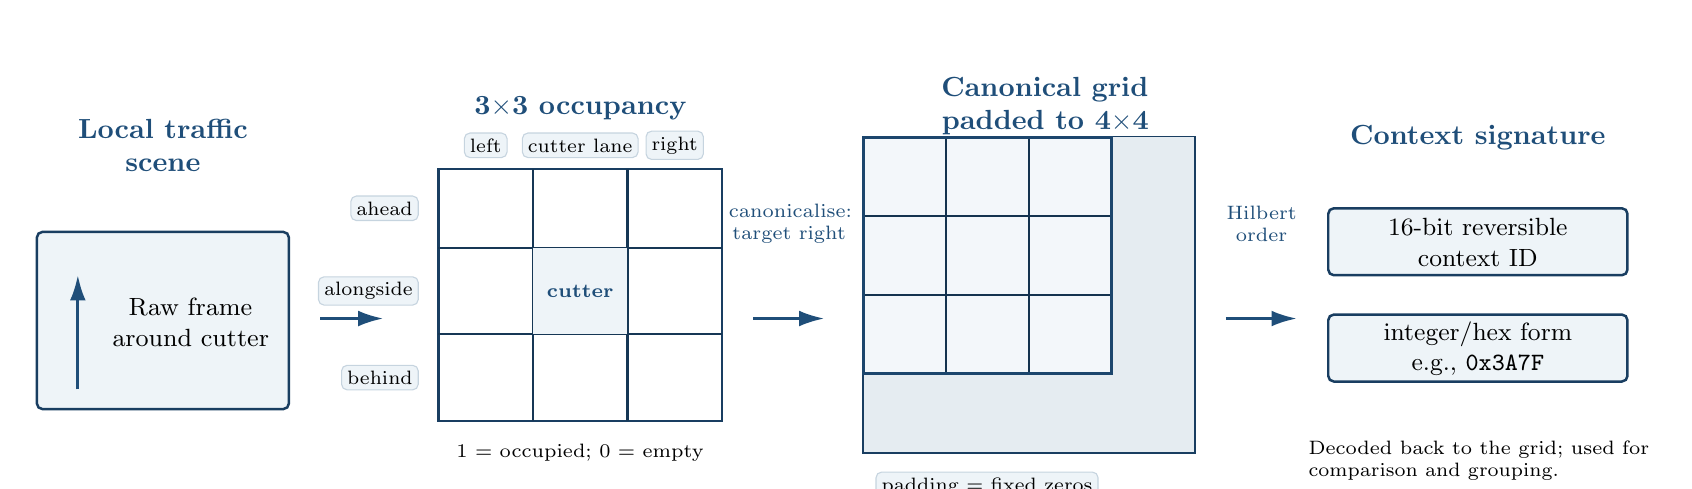
\begin{tikzpicture}[
            x=1cm,y=1cm,>=Latex,font=\small,
            paneltitle/.style={font=\bfseries, align=center, text=accent},
            stagebox/.style={rounded corners=2pt, draw=accent!80!black, line width=0.9pt, fill=accentsoft},
            chip/.style={rounded corners=2pt, draw=accentline, fill=accentsoft, inner sep=2pt, font=\scriptsize},
            arr/.style={-{Latex[length=3.2mm,width=2.0mm]}, line width=1.0pt, draw=accent}
        ]
            % scene
            \node[paneltitle, text width=3.2cm] at (1.7,4.35) {Local traffic\\scene};
            \draw[stagebox] (0.1,1.0) rectangle (3.3,3.25);
            \node[align=center, text width=2.1cm] at (2.05,2.10) {Raw frame\\around cutter};
            \draw[arr] (0.62,1.25) -- (0.62,2.70);

            % arrow 1
            \draw[arr] (3.7,2.15) -- (4.5,2.15);

            % 3x3 grid
            \node[paneltitle, text width=4.2cm] at (7.0,4.82) {3$\times$3 occupancy};
            \draw[draw=accent!80!black, line width=1.0pt] (5.2,0.85) rectangle (8.8,4.05);
            \foreach \x in {6.4,7.6} {\draw[draw=accent!70!black, line width=0.8pt] (\x,0.85) -- (\x,4.05);}
            \foreach \y in {1.95,3.05} {\draw[draw=accent!70!black, line width=0.8pt] (5.2,\y) -- (8.8,\y);}
            \fill[accentsoft] (6.4,1.95) rectangle (7.6,3.05);
            \node[font=\scriptsize\bfseries, align=center, text=accent] at (7.0,2.5) {cutter};
            \node[chip] at (5.8,4.35) {left};
            \node[chip] at (7.0,4.35) {cutter lane};
            \node[chip] at (8.2,4.35) {right};
            \node[chip, anchor=east] at (4.95,3.55) {ahead};
            \node[chip, anchor=east] at (4.95,2.50) {alongside};
            \node[chip, anchor=east] at (4.95,1.40) {behind};
            \node[font=\scriptsize, align=center, text width=4.0cm] at (7.0,0.45) {$1$ = occupied; $0$ = empty};

            % arrow 2
            \draw[arr] (9.2,2.15) -- (10.1,2.15);
            \node[font=\scriptsize, align=center, text=accent, text width=2.0cm] at (9.65,3.35) {canonicalise:\\target right};

            % 4x4 grid
            \node[paneltitle, text width=4.4cm] at (12.9,4.85) {Canonical grid padded to 4$\times$4};
            \fill[lightfill] (10.6,0.45) rectangle (14.8,4.45);
            \draw[draw=accent!80!black, line width=0.9pt] (10.6,0.45) rectangle (14.8,4.45);
            \foreach \x in {11.65,12.7,13.75} {\draw[draw=accent!65!black, line width=0.8pt] (\x,0.45) -- (\x,4.45);}
            \foreach \y in {1.45,2.45,3.45} {\draw[draw=accent!65!black, line width=0.8pt] (10.6,\y) -- (14.8,\y);}
            \fill[accentline!45] (10.6,0.45) rectangle (11.65,1.45);
            \fill[accentline!45] (11.65,0.45) rectangle (12.7,1.45);
            \fill[accentline!45] (12.7,0.45) rectangle (13.75,1.45);
            \fill[accentline!45] (13.75,0.45) rectangle (14.8,1.45);
            \fill[accentline!45] (13.75,1.45) rectangle (14.8,2.45);
            \fill[accentline!45] (13.75,2.45) rectangle (14.8,3.45);
            \fill[accentline!45] (13.75,3.45) rectangle (14.8,4.45);
            \draw[draw=accent!90!black, line width=1.0pt] (10.6,1.45) rectangle (13.75,4.45);
            \node[chip, anchor=west] at (10.75,0.02) {padding = fixed zeros};

            % arrow 3
            \draw[arr] (15.2,2.15) -- (16.1,2.15);
            \node[font=\scriptsize, align=center, text=accent, text width=1.9cm] at (15.65,3.35) {Hilbert\\order};

            % code boxes
            \node[paneltitle, text width=4.4cm] at (18.4,4.45) {Context signature};
            \draw[stagebox] (16.5,2.7) rectangle (20.3,3.55);
            \node[align=center] at (18.4,3.12) {16-bit reversible\\context ID};
            \draw[stagebox] (16.5,1.35) rectangle (20.3,2.2);
            \node[align=center] at (18.4,1.77) {integer/hex form\\e.g., \texttt{0x3A7F}};
            \node[font=\scriptsize, align=left, text width=4.4cm] at (18.45,0.35) {Decoded back to the grid; used for comparison and grouping.};
        \end{tikzpicture}%
        }
        \caption{Construction of an interaction context signature. The first panel is the cutter-centred local scene for one frame; the vertical arrow defines the forward/ahead direction. The scene is discretised into 3$\times$3 occupancy cells, mirrored to a common target-right orientation, padded with fixed zero cells to a 4$\times$4 grid, and read in Hilbert order as a reversible 16-bit context code. The code identifies the local traffic layout; it is not a risk score.}
        \label{fig:sfc-signature-overview}
    \end{figure}

    We perform an exhaustive round-trip test across all $2^{16}$ possible bit patterns because the later code-level agreement checks are only meaningful if the encoding is lossless. The result confirms reversibility: encoding followed by decoding returns the original grid for both Hilbert and Morton (Z-order) traversals.

% ==============================================================================
    \chapter{Methods}
    \label{chap:methods}

    \section{Framework overview}
    \FrameworkName{} starts from trajectories, vehicle geometry, and lane-marking metadata. From these inputs it reconstructs lane assignments, neighbour relations, cut-in events, pair-specific safety indicators, and context signatures. For evaluation, the same downstream analysis is run in two parallel paths:

    \begin{itemize}[leftmargin=1.2em]
  \item \textbf{Reference-label path:} uses highD-provided lane and neighbour identifiers to produce reference relations, events, and signatures.
  \item \textbf{Reconstruction path:} uses only trajectories and lane markings to produce the same outputs without using highD's derived relational fields as inputs.
    \end{itemize}

    This two-path design enables like-for-like agreement measurements at the frame, event, and representation levels. Figure~\ref{fig:framework-overview} summarises the processing flow and highlights the evaluation boundary. Table~\ref{tab:framework-phases} presents the same pipeline as a compact phase/output summary so that the main artefacts can be located quickly in the later results chapter.

    \begin{figure}[p]
        \centering
        \captionsetup{width=0.97\linewidth}
        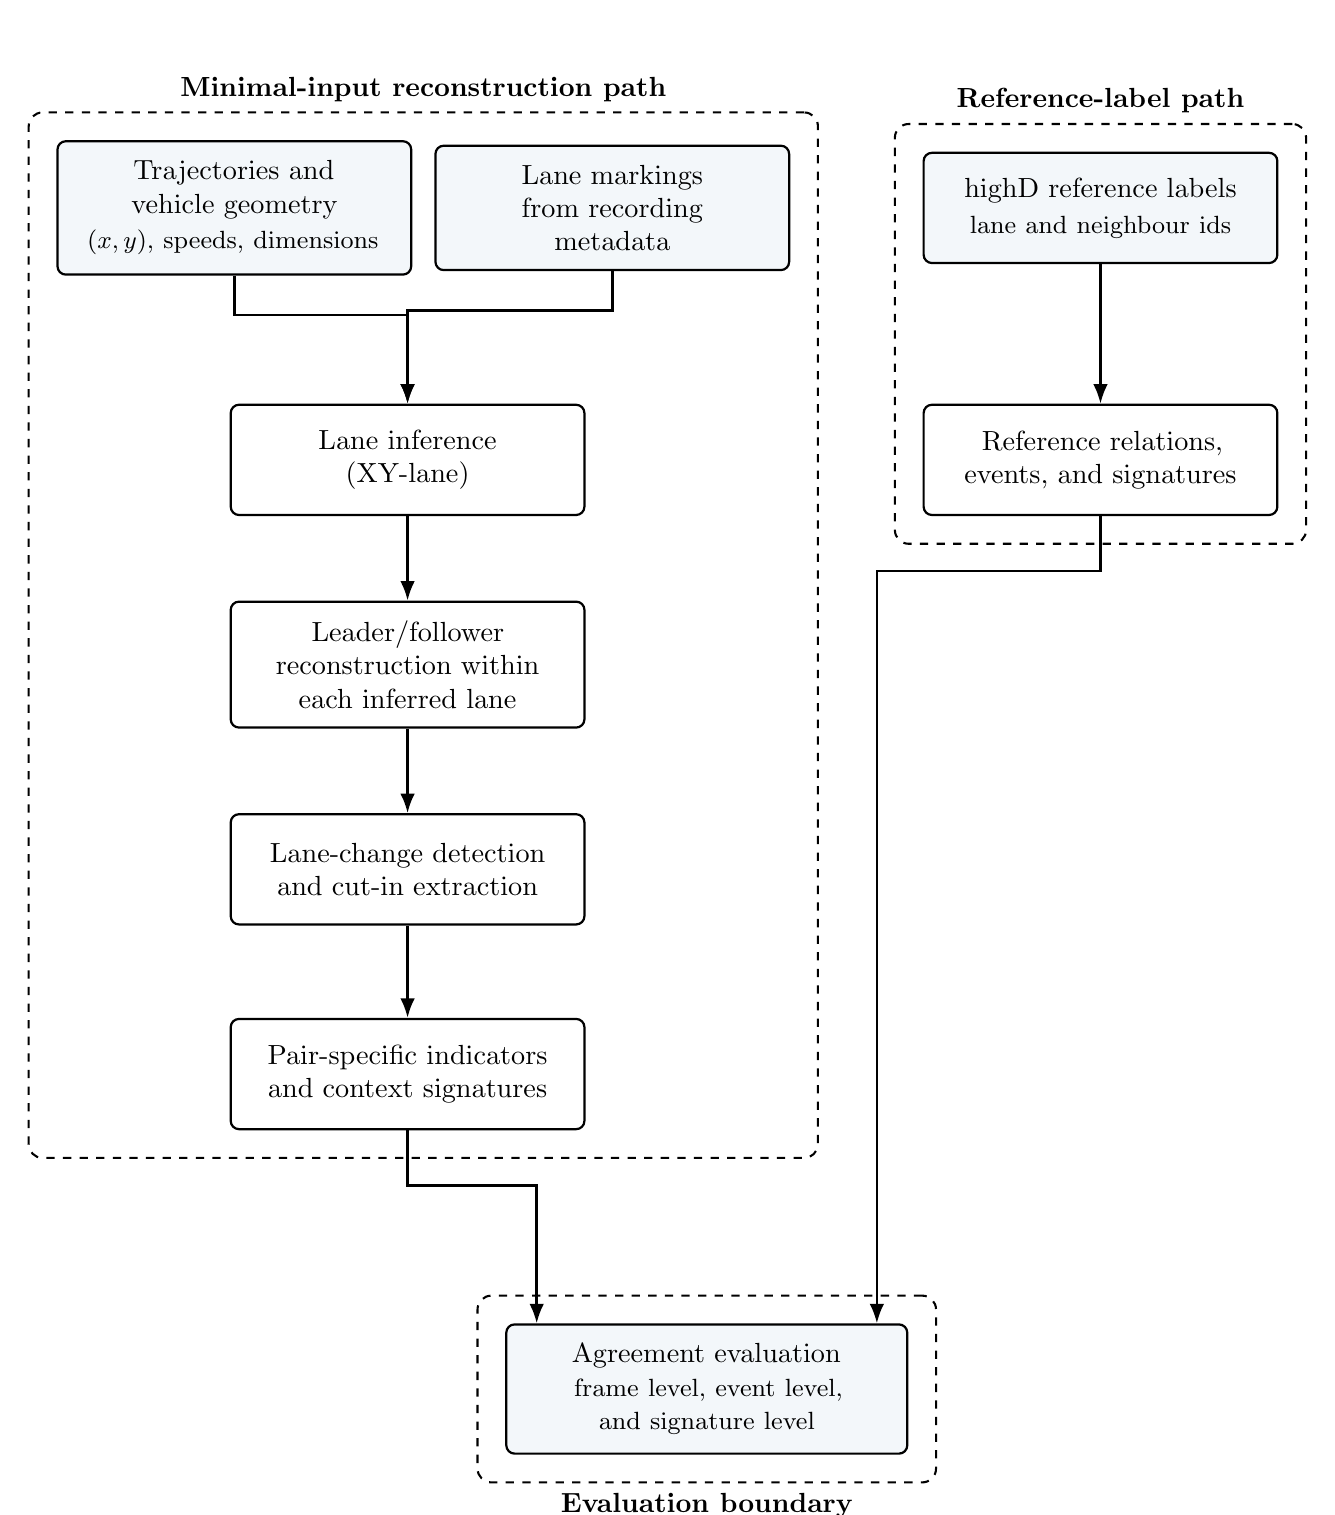
\begin{tikzpicture}[
            font=\normalsize,
            >=Latex,
            % --- node styles ---
            inputblock/.style={
                draw, rounded corners=3pt, line width=0.8pt,
                minimum height=14mm, text width=40mm,
                align=center, inner sep=7pt,
                fill=lightfill
            },
            block/.style={
                draw, rounded corners=3pt, line width=0.8pt,
                minimum height=14mm, text width=40mm,
                align=center, inner sep=7pt
            },
            evalblock/.style={
                draw, rounded corners=3pt, line width=0.8pt,
                minimum height=15mm, text width=46mm,
                align=center, inner sep=7pt,
                fill=lightfill
            },
            % --- edge style ---
            arr/.style={->, line width=0.9pt},
            % --- group style ---
            group/.style={
                draw, rounded corners=5pt, dashed,
                line width=0.75pt, inner sep=10pt
            },
            grouplabel/.style={
                font=\normalsize\bfseries
            }
        ]

        % ============================================================
        %  Layout: two inputs at top (x=0, x=5.2), chain centred at
        %  x=2.6 below them;  reference column at x=10.2.
        %  Evaluation centred between columns at bottom.
        %  Text width ≈ 150 mm (A4, 35+25 mm margins).
        % ============================================================

        % --- Row 0: inputs ---
        \node[inputblock] (traj) at (0, 0)
            {Trajectories and\\vehicle geometry\\[1pt]
             {\small $(x,y)$, speeds, dimensions}};

        \node[inputblock] (lanemeta) at (4.8, 0)
            {Lane markings\\from recording\\metadata};

        % --- Reconstruction chain (centred under two inputs) ---
        \node[block] (lane) at (2.2, -3.2)
            {Lane inference\\(XY-lane)};

        \node[block] (neigh) at (2.2, -5.8)
            {Leader/follower\\reconstruction within\\each inferred lane};

        \node[block] (events) at (2.2, -8.4)
            {Lane-change detection\\and cut-in extraction};

        \node[block] (features) at (2.2, -11.0)
            {Pair-specific indicators\\and context signatures};

        % --- Reference path (right column) ---
        \node[inputblock] (reflabels) at (11, 0)
            {highD reference labels\\[1pt]
             {\small lane and neighbour ids}};

        \node[block] (reference) at (11, -3.2)
            {Reference relations,\\events, and signatures};

        % --- Evaluation (centred between columns) ---
        \node[evalblock] (eval) at (6.0, -15.0)
            {Agreement evaluation\\[1pt]
             {\small frame level, event level,\\and signature level}};

        % ===== Arrows: reconstruction path =====
        \draw[arr] (traj.south)     -- ++(0,-0.5) -| (lane);
        \draw[arr] (lanemeta.south) -- ++(0,-0.5) -| (lane);
        \draw[arr] (lane)   -- (neigh);
        \draw[arr] (neigh)  -- (events);
        \draw[arr] (events) -- (features);

        % ===== Arrows: reference path =====
        \draw[arr] (reflabels) -- (reference);

        % ===== Arrows: converging into evaluation =====
        \draw[arr] (features.south) -- ++(0,-0.7) -| ([xshift=4mm]eval.north west);
        \draw[arr] (reference.south) -- ++(0,-0.7) -| ([xshift=-4mm]eval.north east);

        % ===== Grouping boxes =====
        \node[group,
              fit=(traj)(lanemeta)(lane)(neigh)(events)(features),
              label={[grouplabel]above:Minimal-input reconstruction path}
             ] {};

        \node[group,
              fit=(reflabels)(reference),
              label={[grouplabel]above:Reference-label path}
             ] {};

        \node[group,
              fit=(eval),
              label={[grouplabel]below:Evaluation boundary}
             ] {};

        \end{tikzpicture}
        \caption{Overview of \FrameworkName{}. The minimal-input reconstruction path starts from trajectories, vehicle geometry, and lane markings, then reconstructs lanes, same-lane relations, cut-in events, pair-specific indicators, and context signatures. In parallel, a reference-label path derived from highD lane and neighbour identifiers generates comparison outputs that are used only for agreement evaluation.}
        \label{fig:framework-overview}
    \end{figure}


    \begin{table}[H]
        \centering
        \caption{Macro-phases and outputs of \FrameworkName{}.}
        \label{tab:framework-phases}
        {\small
        \setlength{\tabcolsep}{4pt}
            \begin{tabularx}{\textwidth}{@{}l l >{\raggedright\arraybackslash}X@{}}
\toprule
Phase & Component & Main outputs \\
\midrule
Preliminary processing & Data harmonisation & Consolidated per-frame dataset; sanity checks. \\
\midrule
Core reconstruction & XY-lane inference (Traj2Rel) & Predicted lane index $\hat{L}$ per frame from $y$ and lane markings. \\
Core reconstruction & Neighbour reconstruction (Traj2Rel) & Predicted same-lane leader and follower identifiers per frame via within-lane longitudinal ordering. \\
\midrule
Interaction mining & Cut-in event extraction & Cut-in table with explicit cutter--follower pairs and onset $t_0$. \\
Safety quantification & Pair-consistent indicators \& stages & DHW/THW/TTC for the interacting pair; stage-wise aggregates and risk summaries. \\
\midrule
Context signatures & Occupancy \& SFC encoding & Mirror-normalised occupancy matrices; reversible 16-bit SFC context signatures (hex + bits); stage-level context features. \\
\midrule
Reference-label evaluation & Agreement reporting & Frame-level accuracy, event-level precision/recall/$F_1$, and representation-level match/Hamming-distance diagnostics. \\
\bottomrule
            \end{tabularx}}
    \end{table}

    The remainder of this chapter describes each component. Qualitative inspection was additionally performed using an interactive inspection dashboard (Appendix~\ref{app:dashboard}). The dashboard was an internal validation aid used to inspect onset alignment, decoded occupancy, and extreme events; it was not a separate user study or a manual relabelling step.

    \section{Data preparation and relation reconstruction}
    \subsection{Preliminary processing and data harmonisation}
    Each highD recording is distributed as three data tables: (i) per-frame trajectories, (ii) per-vehicle metadata, and (iii) recording-level metadata. In preliminary processing we load these tables, perform basic consistency checks (e.g., frame rate and track bounds), and combine them into a consolidated per-frame dataset where each row corresponds to one vehicle at one time step together with the metadata needed in later phases. This consolidated representation is used by both the reference-label path and the reconstruction path so that subsequent comparisons are like-for-like.

    We also extract lane-marking positions from the recording metadata because they provide the only map-related input used by the reconstruction method. Dataset-provided lane and neighbour identifiers are retained only for evaluation and are never used as inputs in the reconstruction path.

    The next step is the reconstruction layer (Traj2Rel), which derives two pieces of relational information from minimal inputs: (i) lane membership for each vehicle and time step, and (ii) the identity of the closest vehicle ahead and behind in the same lane. Together these relations are sufficient to define leader--follower interactions and to express cut-in events as explicit cutter--follower pairs.

    \subsection{Lane inference from lateral position (XY-lane)}
    Lane membership is inferred by mapping lateral position to the interval between two consecutive lane markings provided in the recording metadata. Values outside the roadway are mapped to lane id 0 and are excluded from interaction mining. Algorithm~\ref{alg:lane-inference} summarises the procedure.

    \begin{algorithm}[b]
\caption{Lane inference from lateral position and lane markings}
\label{alg:lane-inference}
\KwIn{Vehicle lateral position $y(t)$ and lane boundaries $\{b_0,\dots,b_K\}$ from recording metadata.}
\KwOut{Inferred lane index $\ell(t) \in \{1,\dots,K\}$ (or 0 if outside the roadway).}

\ForEach{frame $t$}{
    \If{$y(t) \notin [b_0, b_K)$}{
        $\ell(t) \leftarrow 0$\tcp*{outside valid lanes}
    }
    \Else{
        find $k$ such that $b_{k-1} \le y(t) < b_k$\;
        $\ell(t) \leftarrow k$\;
    }
}
    \end{algorithm}

    \subsection{Same-lane leader/follower reconstruction}
    Within each frame and inferred lane, vehicles are ordered by longitudinal position in the travel direction. The immediate leader (ahead) and follower (behind) are given by adjacent vehicles in this ordering. Algorithm~\ref{alg:neighbor-reconstruction} summarises the procedure.

    \begin{algorithm}[b]
\caption{Same-lane leader/follower reconstruction from geometry}
\label{alg:neighbor-reconstruction}
\KwIn{Frame-wise vehicle states with longitudinal position $x(t)$ and inferred lane index $\ell(t)$.}
\KwOut{For each vehicle: leaderId and followerId in the same lane (or 0 if none).}

\ForEach{frame $t$}{
    group vehicles by lane $\ell$\;
    \ForEach{lane group $\mathcal{V}_{\ell,t}$}{
        sort $\mathcal{V}_{\ell,t}$ by $x(t)$ in travel direction\;
        \ForEach{vehicle $v_i$ in sorted order}{
            leaderId$(v_i) \leftarrow$ closest vehicle ahead in the list (else 0)\;
            followerId$(v_i) \leftarrow$ closest vehicle behind in the list (else 0)\;
        }
    }
}
    \end{algorithm}

    These two components form the core of the \textbf{system under evaluation}: starting from trajectories and lane markings, we can reconstruct the relations needed for downstream interaction mining, indicator computation, and context-signature generation without using dataset-provided neighbour identifiers as inputs.


    \section{Interaction mining}
    \subsection{Lane-change detection}
    A lane change is accepted when a vehicle transitions from one stable lane block to another. In the final highD configuration, stability means that the source lane remains unchanged for at least $N_\text{before}=25$ frames before the transition and the target lane remains unchanged for at least $N_\text{after}=25$ frames after it, corresponding to \SI{1.0}{\second} on each side at \SI{25}{\hertz}. Transitions involving invalid lane identifiers (e.g., lane id 0) are ignored.

    \subsection{Cut-in extraction}
    Given a lane change into target lane $L$ by vehicle $A$:
    \begin{enumerate}[leftmargin=1.6em]
  \item starting from the lane change start, scan frames forward within a fixed search window,
  \item in each frame, identify a vehicle $B$ in lane $L$ for which $A$ is the immediate leader in that frame (according to the chosen source of neighbour relations: reconstructed relations or reference labels),
  \item if the relationship is established within the allowed delay and holds for at least a minimum number of frames, record a cut-in event with cutter $A$, follower $B$, and onset $t_0$ at the first matching frame.
    \end{enumerate}

    Algorithm~\ref{alg:cutin-detection} summarises the rule-based cut-in identification used in the reconstruction and reference-label paths.

    \begin{algorithm}[b]
\caption{Cut-in identification as a cutter--follower pair}
\label{alg:cutin-detection}
\KwIn{Lane-change candidate for vehicle $A$ with target lane $L$, reconstructed relations over time.}
\KwOut{Cut-in event $(A,B,t_0)$ or no event.}

initialise $t_0 \leftarrow \text{undefined}$\;
\ForEach{frame $t$ in a search window after the lane change begins}{
    \If{$A$ is the leader of some vehicle $B$ in lane $L$}{
        set $t_0$ to the first such frame and keep $B$ as follower\;
        \If{the relation $A \rightarrow B$ persists for at least $d_{\min}$ frames}{
            \Return $(A,B,t_0)$\;
        }
    }
}
\Return no event\;
    \end{algorithm}

    \paragraph{Design rationale.}
    The framework separates event extraction from risk labelling. Lane changes are detected between stable segments, which reduces sensitivity to label jitter, and follower pairing requires a minimum persistence duration to avoid one-frame oscillations. This is consistent with naturalistic evidence that cut-ins have non-trivial duration rather than occurring instantaneously~\cite{wang2019cutin}.

    \subsection{Configuration}
    Table~\ref{tab:config} summarises the key parameters used in the final run (highD 01--60, \SI{25}{\hertz}). These parameters are informed by empirical cut-in duration distributions~\cite{wang2019cutin} and the two-phase risk perception model~\cite{zhou2016riskperception}, and are reported to support reproducibility.

    \begin{table}[H]
        \centering
        \caption{Key configuration values for the final framework run.}
        \label{tab:config}
        {\small
        \setlength{\tabcolsep}{4pt}
            \begin{tabularx}{\textwidth}{@{}l l X@{}}
\toprule
Component & Parameter & Value \\
\midrule
Lane-change detection & Min stable before/after & 25 frames ($\approx \SI{1.0}{\second}$) \\
Lane-change detection & Ignored lane ids & \{0\} \\
Cut-in detection & Search window & 50 frames ($\approx \SI{2.0}{\second}$) \\
Cut-in detection & Min relation duration & 10 frames ($\approx \SI{0.4}{\second}$) \\
Cut-in detection & Max relation delay & 15 frames ($\approx \SI{0.6}{\second}$) \\
Indicator computation & Min speed for THW & \SI{0.1}{\meter\per\second} \\
Indicator computation & Closing speed epsilon & $10^{-6}$ \\
Indicator computation & Window (pre/post) for diagnostics & 50/75 frames ($\approx \SI{2}{\second}/\SI{3}{\second}$) \\
Stage model & Total analysis window & $\pm \SI{4}{\second}$ around $t_0$ \\
Risk label & Execution THW threshold & \SI{0.7}{\second} \\
SFC encoding & Ahead/behind range & Disabled (no fixed cutoff) \\
SFC encoding & Alongside threshold & \SI{4.0}{\meter} (final Step 14 thesis run) \\
SFC encoding & Order & Hilbert \\
\bottomrule
            \end{tabularx}}
    \end{table}

    \section{Safety quantification}
    All safety indicators are computed for the explicit cutter--follower pair rather than a generic predecessor, consistent with recent risk models that use interaction-specific features~\cite{shangguan2022,liu2025multitask}. Following Zhou and Itoh~\cite{zhou2016riskperception}, we interpret TTC and THW as complementary indicators across the stage-aligned window.

    We compute DHW/THW/TTC for arbitrary pairs using geometry and speeds. Because trajectory datasets may define position references differently (e.g., centre point vs bounding-box corner), we \emph{select a geometry model} by comparing our computed indicators against highD-provided indicators for same-lane (ego, predecessor) pairs on a large random sample. This calibration step is separate from the reconstruction boundary: highD indicators are used here only as external reference values to choose a consistent position convention, not as hidden inputs to the final cut-in features. We test multiple plausible reference conventions and select the one that best matches dataset-provided DHW/THW/TTC. In the final run, the best match was obtained with a bounding-box--based interpretation of the position variables (a top-left reference point), combined with vehicle length to compute front and rear positions.

    To avoid negative gaps due to noise or reference mismatches, reported minima are clipped to be non-negative for DHW/THW. TTC is treated as infinite when the follower is not closing ($v_B \leq v_A$).

    \subsection{Stage-wise features}
    For each detected cut-in, we align a fixed time window around onset $t_0$ and compute stage-wise summaries for the four stages in Chapter~\ref{chap:theory}. The feature table includes stage minima of DHW/THW/TTC and kinematic aggregates for cutter and follower. These stage-wise summaries are later used not only for descriptive risk analysis, but also for operational-usefulness evaluation through threshold sensitivity and TTC-versus-THW disagreement analysis.

    \subsection{Deceleration-based indicator: DRAC computation}
    \label{sec:drac-method}
    We compute DRAC for the explicit cutter--follower pair in the execution stage using the formula defined in Section~\ref{sec:drac-theory}. The implementation reuses the same pair-consistent longitudinal states (positions, speeds, and DHW) already computed for TTC and THW, so all indicators describe the same interaction pair. DRAC is reported alongside the existing indicators to assess braking demand alongside gap acceptance (THW) and collision timing (TTC).

    \section{Context signatures}
    \label{sec:context-signatures-method}
    To capture local traffic context around the cutter compactly, we encode neighbourhood occupancy into the 3$\times$3 semantic grid defined in Chapter~\ref{chap:theory}. Each frame is mapped to a binary occupancy pattern, and the 3$\times$3 cells are embedded into a 4$\times$4 grid and linearised using a Hilbert-type space-filling-curve order. To remove direction-induced asymmetry, events are mirror-normalised to a canonical orientation prior to aggregation.

    \paragraph{Minimal-input SFC signatures.}
    In the minimal-input path, occupancy is computed from inferred lanes (XY-lane) and lane-snapshot neighbour queries (geometry). This means SFC signatures can be generated without accessing highD neighbour columns.

    \paragraph{Reference SFC signatures.}
    For comparison, we also construct a reference occupancy grid from the highD surrounding-vehicle identifiers (same-lane preceding/following plus left/right neighbours and alongside vehicles). Mapping each non-zero neighbour id to occupancy yields a reference 3$\times$3 grid per frame, which can be encoded into a reference SFC signature.

    \paragraph{Signature agreement.}
    We assess the SFC branch by comparing the reference and minimal-input codes for matching (event, frame) rows. We report both exact code match rate and the distribution of Hamming distances (bitwise differences), which localises whether mismatches affect a single cell or multiple cells.

    \paragraph{Exploratory clustering of decision-stage signatures.}
    As an additional analysis of representational usefulness, we cluster event-level decision-stage context signatures after the core agreement check. For each validated cut-in event, the mirror-normalised decision-stage 3$\times$3 occupancy grids are averaged over the frames in that stage, yielding a 9-dimensional vector of cell-wise occupancy probabilities. We then apply $k$-means clustering for $K=3,\dots,8$, assess internal cohesion with the silhouette score, and assess solution stability with the mean adjusted Rand index (ARI) across repeated random initialisations. This clustering is not used as a primary correctness criterion; it is reported only as an exploratory check of whether the validated SFC representation supports interpretable grouping of decision-stage interaction contexts.

    Algorithm~\ref{alg:sfc-signature} summarises how the context signatures are constructed for each stage-aligned frame.

    \begin{algorithm}[b]
\caption{Cutter-centred occupancy grid and space-filling-curve context signature}
\label{alg:sfc-signature}
\KwIn{Cut-in event $(A,B,t_0)$, reconstructed lane/relations, neighbourhood range parameters.}
\KwOut{A stage-aligned sequence of binary grids and a 16-bit context signature per frame.}

\ForEach{frame $t$ in the analysis window around $t_0$}{
    build a 3$\times$3 cutter-centred occupancy grid around the cutter $A$\;
    (optional) mirror-normalise the grid to a canonical direction\;
    embed the 3$\times$3 grid into a 4$\times$4 grid with fixed padding\;
    traverse cells in Hilbert order and write occupancy bits into a 16-bit code\;
    store the code and (optionally) the decoded grid for inspection\;
}
    \end{algorithm}

    \section{Predictive evaluation: decision-stage risk forecasting}
    \label{sec:risk-prediction-method}
    Beyond descriptive agreement, we evaluate the \emph{predictive value} of the framework's reconstructed features. We test whether features available \emph{before} the cut-in is established (intention and decision stages) can predict execution-stage THW risk (THW$_{\min} < \SI{0.7}{\second}$).

    \paragraph{Feature set.}
    The feature vector used for prediction consists of 34 features: 18 kinematic features from the intention and decision stages (DHW$_{\min}$, THW$_{\min}$, TTC$_{\min}$, cutter/follower speeds, accelerations, and lateral velocity for each stage) and 16 SFC context features (mean occupancy probabilities for each bit position in the decision-stage mirrored Hilbert code).

    \paragraph{Evaluation protocol.}
    We use Leave-One-Recording-Out Cross-Validation (LORO-CV): for each of the 60 recordings, the model is trained on the remaining 59 recordings and tested on the held-out recording. This ensures that all test events come from a traffic environment not seen during training. The classification threshold is optimised on the training fold by maximising $F_1$.

    \paragraph{Model.}
    We train a bagged decision-stump ensemble (50 trees with random feature subsampling), which provides both predictions and feature-importance estimates via Gini gain. The choice of a shallow ensemble rather than a deeper model (e.g., gradient boosting or neural network) is deliberate: with 34 features, 10,023 events, and a 20\% minority class, a high-capacity model risks overfitting to recording-specific artefacts. A decision-stump ensemble offers stable feature-importance rankings for interpretability and has low variance under the 60-fold LORO-CV protocol. The goal of RQ4 is to test whether the reconstructed features carry predictive value at all, not to maximise classification accuracy; a simple model that clearly exceeds the baseline provides stronger evidence for this claim than a tuned model whose performance is harder to attribute to the features alone.

    \paragraph{Baseline.}
    The majority-class baseline assigns the most frequent training-set label to all test events. Because the minority class (risky, 20.1\%) is never the majority, the baseline predicts ``non-risky'' for all events and achieves $F_1 = 0$ for the risky class.

    \paragraph{Ablation.}
    To isolate the contribution of SFC context features versus kinematic indicators, we run the same LORO-CV protocol on three feature subsets: all features (34), kinematic features only (18), and SFC features only (16).

    Unless otherwise noted, uncertainty intervals on reconstruction metrics are computed over the 60 recording-level scores rather than over individual frames. We report these as 95\% normal-approximation intervals for the mean ($\bar{x} \pm 1.96\,\mathrm{SE}$), so that recordings rather than frames act as the unit of aggregation.

    \section{Reproducibility}
    All results reported in this thesis can be regenerated from the released pipeline given the configuration in Table~\ref{tab:config} and the \textit{highD} dataset. Some substeps use stochastic procedures (random sampling for geometry calibration, repeated $k$-means initialisations, and random feature subsampling in the ensemble model), so exact numerical replication additionally requires the same random seeds. The complete pipeline, including scripts for all tables and figures, is publicly available at \ArtifactURL.

% ==============================================================================
    \chapter{Results}
    \label{chap:results}

    \section{Event extraction and dataset overview}
    The final run processes all 60 highD recordings. From 11,856 detected lane changes, the framework extracts 10,026 cut-in events (84.6\%), of which 10,023 remain after stage-window validity checks. The three excluded events are those for which the full stage-aligned feature window falls outside the available track boundaries. Table~\ref{tab:events} summarises the event yield, and Table~\ref{tab:duration-stats} reports duration statistics.

    \begin{table}[H]
        \centering
        \caption{Event counts for the final run (recordings 01--60).}
        \label{tab:events}
        {\small
        \setlength{\tabcolsep}{4pt}
            \begin{tabularx}{\textwidth}{@{}>{\raggedright\arraybackslash}p{0.36\textwidth}rr>{\raggedright\arraybackslash}p{0.34\textwidth}@{}}
\toprule
Artefact & \shortstack{Lane\\changes} & \shortstack{Cut\\-ins} & Notes \\
\midrule
Interaction mining & 11,856 & 10,026 & Extracted from reconstructed relations. \\
Stage feature table & -- & 10,023 & After removing 3 events whose full stage window falls outside the available track range. \\
Context signatures & -- & 1,421,980 & Frame-level signatures for 10,023 events. \\
\bottomrule
            \end{tabularx}
        }
    \end{table}

    \begin{table}[H]
        \centering
        \caption{Duration statistics (highD 01--60, \SI{25}{\hertz}).}
        \label{tab:duration-stats}
        {\small
        \setlength{\tabcolsep}{4pt}
            \begin{tabular}{@{}lrrrrrr@{}}
                \toprule
                Event type & Min (s) & P25 (s) & Median (s) & Mean (s) & P75 (s) & Max (s) \\
                \midrule
                Lane change duration & 0.960 & 3.680 & 6.240 & 6.551 & 8.960 & 69.120 \\
                \shortstack[l]{Observed cut-in relation duration\\within post-onset window} & 0.360 & 1.960 & 1.960 & 1.870 & 1.960 & 1.960 \\
                \bottomrule
            \end{tabular}}

    \vspace{2pt}
    {\footnotesize \emph{Note:} The cut-in relation duration is right-censored by the fixed post-onset extraction window, so the repeated upper quantiles at \SI{1.96}{\second} reflect the event-extraction design rather than an unconstrained natural duration distribution.}
    \end{table}

    \section{Reconstruction accuracy (RQ1/RQ2)}
    Geometry-based same-lane neighbour reconstruction matches highD reference relations with mean accuracy 0.999997. When lane membership is also inferred from geometry (XY-lane), agreement remains high: mean preceding/following accuracy 0.999810/0.999811 (mismatch rate $\approx$0.02\%). Cut-in detection from reconstructed relations matches reference events with $F_1 = 0.998938$, with recording-level 95\% intervals of $\pm 2.3\times10^{-5}$ for neighbour accuracy and $\pm 7.3\times10^{-4}$ for cut-in $F_1$.

    These results establish that the minimal-input path reproduces the reference-label path with high accuracy, validating the reconstruction as a basis for downstream analysis.

    \section{Execution-stage indicator distributions}
    Table~\ref{tab:exec-dist} summarises execution-stage minima across all 10,023 events. TTC statistics are shown only for events with finite TTC (i.e., closing speed).

    \begin{table}[H]
        \centering
        \caption{Execution-stage indicator minima across all events (10,023 cut-ins).}
        \label{tab:exec-dist}
        {\small
        \setlength{\tabcolsep}{4pt}
            \begin{tabular}{@{}lrrrrrr@{}}
                \toprule
                Indicator & Min & P25 & Median & Mean & P75 & Max \\
                \midrule
                DHW$_{\min}$ (m) & 1.37 & 20.69 & 32.21 & 51.28 & 59.82 & 373.98 \\
                THW$_{\min}$ (s) & 0.051 & 0.769 & 1.194 & 1.700 & 2.028 & 12.383 \\
                TTC$_{\min}$ (s), finite only (n=3,606) & 0.220 & 10.769 & 19.726 & 74.161 & 42.025 & 14428.50 \\
                \bottomrule
            \end{tabular}}
    \end{table}

    The TTC distribution is strongly right-skewed, so the median and quartiles are more informative than the mean for interpreting the typical severity of finite-closing events.

    \section{Risk characterisation (RQ2)}
    Using the risk label defined in Chapter~\ref{chap:theory} (execution-stage THW$_{\min} < \SI{0.7}{\second}$), 2,018 of 10,023 events (20.1\%) are classified as risky. Table~\ref{tab:risk-summary} compares the two groups, and Table~\ref{tab:effect-sizes} reports effect sizes using Cliff's $\delta$.

    \begin{table}[H]
        \centering
        \caption{Execution-stage risk summary. $\Delta v = \bar v_{\text{cutter}}-\bar v_{\text{follower}}$.}
        \label{tab:risk-summary}
        {\small
        \setlength{\tabcolsep}{4pt}
            \begin{tabular}{@{}lrrrr@{}}
                \toprule
                Group & Events & THW$_{\min}$ median (s) & DHW$_{\min}$ median (m) & $\Delta v$ median (\si{\meter\per\second}) \\
                \midrule
                Non-risky & 8,005 & 1.427 & 39.680 & 2.304 \\
                Risky & 2,018 & 0.539 & 14.945 & 2.853 \\
                \bottomrule
            \end{tabular}}
    \end{table}

    \begin{table}[H]
        \centering
        \caption{Effect sizes between risk groups (execution stage). $\delta$ is Cliff's delta.}
        \label{tab:effect-sizes}
        \begin{tabular}{@{}lrrr@{}}
            \toprule
            Metric & Median non-risky & Median risky & Cliff's $\delta$ \\
            \midrule
            DHW$_{\min}$ (\si{\meter}) & 39.68 & 14.95 & $-0.950$ \\
            $\Delta v$ (\si{\meter\per\second}) & 2.304 & 2.853 & $0.032$ \\
            $\lvert v_{y,\text{cutter}}\rvert_{\max}$ (\si{\meter\per\second}) & 0.88 & 0.93 & $0.097$ \\
            \bottomrule
        \end{tabular}
    \end{table}

    The large effect size for DHW$_{\min}$ ($\delta = -0.950$) is expected given the direct relationship $\mathrm{THW}=\mathrm{DHW}/v_B$. The negligible effect for lateral velocity ($\delta = 0.097$) indicates that the THW-based label captures longitudinal gap acceptance rather than lateral kinematics.

    \paragraph{Threshold sensitivity.}
    Table~\ref{tab:sensitivity} shows how risk prevalence varies with the THW threshold, ranging from 7.58\% at \SI{0.50}{\second} to 62.21\% at \SI{1.50}{\second}. Across the 60 recordings, the risk ratio varies between 11.1\% and 34.1\% (median 20.0\%).

    \begin{table}[H]
        \centering
        \caption{THW threshold sensitivity (10,023 events).}
        \label{tab:sensitivity}
        \begin{tabular}{@{}lrr@{}}
            \toprule
            THW threshold (s) & Risky events & Prevalence \\
            \midrule
            0.50 & 760 & 7.58\% \\
            0.70 & 2,018 & 20.13\% \\
            1.00 & 4,004 & 39.95\% \\
            1.50 & 6,235 & 62.21\% \\
            \bottomrule
        \end{tabular}
    \end{table}

    \section{Multi-indicator analysis (RQ2)}
    \label{sec:drac-results}

    \paragraph{Indicator complementarity: THW, TTC, and DRAC.}
    The three indicators capture fundamentally different aspects of cut-in severity. TTC is finite for only 3,606 of 10,023 events (35.98\%), meaning that a TTC-only analysis would miss the majority of established interactions. DRAC is finite for a similar share (3,393 events, 33.9\%), but its median value is \SI{0.071}{\meter\per\second\squared}, which is well below any critical threshold. Only 8 events (0.08\%) exceed the hard-braking threshold of \SI{3.35}{\meter\per\second\squared}. In contrast, THW flags 20.1\% of events as risky. Tables~\ref{tab:drac-dist}--\ref{tab:ttc-thw-overlap} detail these distributions.

    \begin{table}[H]
        \centering
        \caption{Execution-stage DRAC distribution (finite only, $n=3{,}393$).}
        \label{tab:drac-dist}
        {\small
            \begin{tabular}{@{}lrrrrrr@{}}
                \toprule
                Indicator & Min & P25 & Median & Mean & P75 & P95 \\
                \midrule
                DRAC (\si{\meter\per\second\squared}) & $<$0.001 & 0.016 & 0.071 & 0.193 & 0.202 & 0.693 \\
                \bottomrule
            \end{tabular}}
    \end{table}

    \begin{table}[H]
        \centering
        \caption{DRAC threshold sensitivity (10,023 events).}
        \label{tab:drac-sensitivity}
        \begin{tabular}{@{}lrr@{}}
            \toprule
            DRAC threshold (\si{\meter\per\second\squared}) & Flagged events & Ratio \\
            \midrule
            1.0  &  80  &  0.80\% \\
            2.0  &  18  &  0.18\% \\
            3.0  &   9  &  0.09\% \\
            3.35 &   8  &  0.08\% \\
            5.0  &   6  &  0.06\% \\
            \bottomrule
        \end{tabular}
    \end{table}

    \begin{table}[H]
        \centering
        \caption{Execution-stage TTC by THW risk group (finite TTC only, $n=3{,}606$).}
        \label{tab:ttc-finite}
        \begin{tabular}{@{}lrrr@{}}
            \toprule
            Group (by THW label) & Events & TTC median (s) & TTC mean (s) \\
            \midrule
            Non-risky & 3,177 & 22.30 & 80.27 \\
            Risky & 429 & 8.98 & 28.94 \\
            \bottomrule
        \end{tabular}
    \end{table}

    \begin{table}[H]
        \centering
        \caption{THW-risky vs TTC-threshold overlap (infinite TTC counted as not risky).}
        \label{tab:ttc-thw-overlap}
        \begin{tabular}{@{}rrrrrr@{}}
            \toprule
            TTC thr. (s) & TTC-flagged & TP & FP & Prec. & Rec. \\
            \midrule
            1.5 & 10 & 10 & 0 & 1.000 & 0.005 \\
            3.0 & 43 & 37 & 6 & 0.860 & 0.018 \\
            5.0 & 156 & 99 & 57 & 0.635 & 0.049 \\
            10.0 & 788 & 237 & 551 & 0.301 & 0.117 \\
            \bottomrule
        \end{tabular}
    \end{table}

    These results show that no single indicator captures all aspects of cut-in severity. THW identifies short accepted gaps, TTC captures closing-speed conflicts, and DRAC quantifies braking demand. The framework's pair-consistent computation makes this multi-indicator perspective possible because all measures describe the same cutter--follower interaction~\cite{zhou2016riskperception,wang2021ssm}.

    \paragraph{Extreme events.}
    Table~\ref{tab:top-ttc} lists the three events with the lowest finite TTC, useful for qualitative inspection (Appendix~\ref{app:dashboard}).

    \begin{table}[H]
        \centering
        \caption{Top-3 extreme events by minimum execution-stage TTC (finite only).}
        \label{tab:top-ttc}
        \begin{tabular}{@{}rrrrrrr@{}}
            \toprule
            Rec. & Cutter & Follower & From & To & TTC$_{\min}$ (s) & THW$_{\min}$ (s) \\
            \midrule
            40 & 682 & 687 & 1 & 2 & 0.220 & 0.051 \\
            26 & 496 & 522 & 1 & 2 & 0.235 & 0.122 \\
            30 & 839 & 852 & 1 & 2 & 0.288 & 0.067 \\
            \bottomrule
        \end{tabular}
    \end{table}

    \section{Context signature maps and interpretation}
    \label{sec:context-maps}
    This section decodes the mirrored SFC signatures from Section~\ref{sec:context-signatures-method} back into the underlying semantic 3$\times$3 occupancy grid so that the spatial meaning of the codes becomes visible. For each stage-aligned frame, each cell is binary ($1$ if at least one vehicle occupies that semantic region, else $0$); the plotted cell values are then simple group means:
    \[
        \bar{G}_{r,c} = \frac{1}{N}\sum_{i=1}^{N} G^{(i)}_{r,c},
    \]
    where $G^{(i)}_{r,c}\in\{0,1\}$ is the occupancy of cell $(r,c)$ in one mirrored stage frame. Each number in Figures~\ref{fig:sfc-decision-grids}--\ref{fig:sfc-archetypes} should therefore be read as a \emph{mean occupancy probability}. For example, a value of 60\% in one cell means that the corresponding semantic region is occupied in 60\% of the relevant stage frames.

    After mirror normalisation, the left column corresponds to the lane \emph{away from the manoeuvre}, the middle column to the cutter's current lane, and the right column to the \emph{target lane}. The rows should be read top-to-bottom as \emph{ahead}, \emph{alongside}, and \emph{behind} the cutter. The centre cell is not analytically informative because the cutter itself occupies it by construction; it is therefore shown as fixed rather than interpreted as evidence about surrounding traffic.

    We present the decision stage as a representative example because it captures the traffic configuration immediately before the cut-in interaction becomes established. Figure~\ref{fig:sfc-decision-grids} therefore shows both absolute occupancy maps (non-risk and risky) and the risk-minus-non-risk difference map for the decision stage. The absolute maps provide context; the difference map is the main analytical view and is computed cell-wise as
    \[
        \Delta_{r,c}^{\mathrm{pp}} = 100\left(\bar{G}^{\text{risk}}_{r,c} - \bar{G}^{\text{non-risk}}_{r,c}\right),
    \]
    measured in \emph{percentage points} (pp). Thus, a label of $+3.2$ pp means that the cell is occupied 3.2 percentage points more often in risky events, while $-5.6$ pp means that the same cell is occupied 5.6 percentage points more often in non-risk events.

    To highlight how group differences evolve over time, Figure~\ref{fig:sfc-stage-diff} shows risk-minus-non-risk difference maps for the intention, decision, and execution stages using a consistent zero-centred colour scale. The key point is not that risky and non-risky cut-ins form completely different scene types; rather, they share a common cut-in geometry and differ through comparatively small occupancy shifts in a few neighbouring cells. This is why the absolute maps look broadly similar and why the difference maps are more informative.

    \begin{figure}[H]
        \centering
        \safeincludegraphics[width=0.43\textwidth]{decision_nonrisk.png}\hfill
        \safeincludegraphics[width=0.43\textwidth]{decision_risk.png}\\[5pt]
        \safeincludegraphics[width=0.62\textwidth]{decision_diff.png}
        \caption{Decision-stage occupancy maps. The top panels show cell-wise mean occupancy probabilities for non-risk and risky events after mirror normalisation, so each label is the share of decision-stage frames in which that semantic cell is occupied. The bottom panel shows the cell-wise difference (risk minus non-risk) in percentage points.}
        \label{fig:sfc-decision-grids}
    \end{figure}

    \begin{figure}[p]
        \centering
        \textbf{Intention stage}\\[2pt]
        \safeincludegraphics[width=0.50\textwidth]{intention_diff.png}\\[6pt]
        \textbf{Decision stage}\\[2pt]
        \safeincludegraphics[width=0.50\textwidth]{decision_diff.png}\\[6pt]
        \textbf{Execution stage}\\[2pt]
        \safeincludegraphics[width=0.50\textwidth]{execution_diff.png}
        \caption{Stage-wise risk-minus-non-risk occupancy differences for the intention, decision, and execution stages, shown separately to make the small cell-wise shifts easier to read. Red indicates cells occupied more often in risky events, blue indicates the opposite, and each signed label is a percentage-point difference (pp). The centre cell is neutral because the cutter occupies it by construction.}
        \label{fig:sfc-stage-diff}
    \end{figure}

    In practical terms, these plots should be read as subtle but structured differences in local traffic context. They suggest that the risky group is associated not with an entirely separate scene family, but with small changes in how tightly neighbouring cells around the cutter are occupied during the lead-up to the cut-in. A compact reading is that risky events shift occupancy away from cells \emph{ahead} of the cutter and toward cells \emph{alongside} or \emph{behind} it during the intention and decision stages; by the execution stage, the remaining differences are smaller and are concentrated mainly in the cells behind the manoeuvre. In the decision stage, the most meaningful pattern is therefore a modest tightening around the target-lane gap rather than a wholesale change of scene type, which is consistent with risky cut-ins being executed in more constrained surrounding traffic.

    \subsection{Exploratory decision-stage context archetypes}
    Mean occupancy maps show group-level differences, but they do not directly answer whether the validated SFC representation can recover a small set of reusable scene families. As an additional representational-usefulness check, we therefore decode the mirrored binary SFC signatures back into the semantic 3$\times$3 grid, average the decision-stage grids within each event, and cluster the resulting event-level context vectors. We use the \emph{decision} stage rather than the execution stage so that clustering is based on decision-stage context rather than on the same time window used to define the THW risk label.

    Searching $K=3,\dots,8$ with $k$-means, the best solution is $K=7$, with silhouette score 0.498 and mean stability ARI 0.976 across repeated initialisations. The resulting archetypes remain reasonably balanced, spanning 6.0\%--30.7\% of all 10,023 validated cut-ins. The labels A1--A7 in Figure~\ref{fig:sfc-archetypes} are therefore \emph{cluster identifiers}, not manually defined classes; they are relabelled by cluster size so that A1 is the largest archetype and A7 the smallest. Each panel reports four things at once: the mean occupancy probabilities for that cluster, the cluster's share of all events, its execution-stage THW-risk prevalence, and its risk ratio relative to the overall 20.13\% risk prevalence.

    Figure~\ref{fig:sfc-archetypes} shows the seven archetypes, and Figure~\ref{fig:sfc-archetype-risk} compares their execution-stage THW risk prevalence. Read qualitatively, A1 and A2 are leader-dominated patterns with strong occupancy ahead of the cutter, A3 combines strong leaders ahead with a frequent target-lane follower, A4 represents the tightest target-lane corridor (high occupancy both ahead of and behind the target gap), A5 is follower-dominated in the cutter/target lanes, A6 concentrates traffic mainly ahead across all lanes, and A7 is dominated by followers behind the cutter across all three lanes. The most risk-enriched archetype (A4, 10.27\% of events) reaches 26.63\% risky outcomes versus 20.13\% overall (risk ratio 1.32) with median execution THW \SI{0.975}{\second}. Lower-risk archetypes such as A2 and A6 remain below the overall prevalence (17.55\% and 16.29\%, respectively). The SFC code therefore supports interpretable unsupervised grouping of cut-in scenes based on decision-stage context.

    \begin{figure}[p]
        \centering
        \safeincludegraphics[width=0.97\textwidth,height=0.72\textheight,keepaspectratio]{archetype_heatmaps.png}
        \caption{Seven decision-stage context archetypes derived from mirrored binary SFC signatures. A1--A7 are unsupervised cluster IDs relabelled by cluster size (A1 largest). In each panel, cell labels show mean occupancy percentages, while the text above the grid reports the archetype's event share, risk prevalence, and risk ratio relative to the overall dataset. The grey hatched centre cell is neutralised because the cutter occupies it by construction.}
        \label{fig:sfc-archetypes}
    \end{figure}

    \begin{figure}[H]
        \centering
        \safeincludegraphics[width=0.70\textwidth]{archetype_risk_prevalence.png}
        \caption[THW risk prevalence by context archetype]{Execution-stage THW risk prevalence by decision-stage context archetype.}
        \label{fig:sfc-archetype-risk}
    \end{figure}

    \section{Predictive evaluation (RQ4)}
    \label{sec:risk-prediction-results}

    Table~\ref{tab:prediction-summary} summarises the LORO-CV results for the decision-stump ensemble on the full feature set.

    \begin{table}[H]
        \centering
        \caption{Risk prediction: LORO-CV summary (stump ensemble, 34 features from the intention and decision stages, 60 held-out folds).}
        \label{tab:prediction-summary}
        \begin{tabular}{@{}lrl@{}}
            \toprule
            Metric & Mean & $\pm$ Std \\
            \midrule
            ROC-AUC       & 0.822 & $\pm 0.058$ \\
            $F_1$ (risky class) & 0.506 & $\pm 0.088$ \\
            Precision     & 0.357 & $\pm 0.083$ \\
            Recall        & 0.907 & $\pm 0.060$ \\
            Baseline $F_1$     & 0.000 & $\pm 0.000$ \\
            $\Delta F_1$ vs baseline & +0.506 & $\pm 0.088$ \\
            \bottomrule
        \end{tabular}
    \end{table}

    The model achieves ROC-AUC of 0.82, indicating good discriminative ability between risky and non-risky events based on features available before the execution stage. The high recall (0.91) means the model identifies most risky events before the execution stage, while the lower precision (0.36) reflects false positives: events that appear risky based on decision-stage features but resolve safely. This asymmetry is expected because not all tight decision-stage gaps lead to risky outcomes; follower adaptation and cutter acceleration can widen the gap during execution.

    \paragraph{Feature importance.}
    Table~\ref{tab:feature-importance} lists the five most important features by Gini importance.

    \begin{table}[H]
        \centering
        \caption{Top-5 features by Gini importance (stump ensemble, LORO-CV).}
        \label{tab:feature-importance}
        \begin{tabular}{@{}lr@{}}
            \toprule
            Feature & Importance \\
            \midrule
            Decision-stage THW$_{\min}$  & 0.268 \\
            Decision-stage DHW$_{\min}$  & 0.247 \\
            Intention-stage DHW$_{\min}$ & 0.119 \\
            Intention-stage THW$_{\min}$ & 0.110 \\
            Decision-stage TTC$_{\min}$  & 0.055 \\
            \bottomrule
        \end{tabular}
    \end{table}

    Decision-stage DHW and THW minima together account for about 52\% of the total importance, which confirms that gap acceptance in the decision stage is the strongest predictor of execution-stage risk. Among the SFC features, the two most informative bits (SFC positions 13 and 8) contribute modestly, suggesting that specific occupancy configurations carry additional predictive information.

    \paragraph{Ablation study.}
    Table~\ref{tab:ablation} compares models trained on different feature subsets.

    \begin{table}[H]
        \centering
        \caption{Feature ablation: LORO-CV (stump ensemble).}
        \label{tab:ablation}
        \begin{tabular}{@{}lrll@{}}
            \toprule
            Feature set & $n$ & Mean AUC ($\pm$ std) & Mean $F_1$ ($\pm$ std) \\
            \midrule
            All (kinematic + SFC) & 34 & 0.822 ($\pm 0.058$) & 0.506 ($\pm 0.088$) \\
            Kinematic only        & 18 & 0.832 ($\pm 0.061$) & 0.519 ($\pm 0.086$) \\
            SFC only              & 16 & 0.621 ($\pm 0.059$) & 0.349 ($\pm 0.056$) \\
            \bottomrule
        \end{tabular}
    \end{table}

    Kinematic features alone achieve a slightly higher AUC (0.832) than the full model (0.822), while the SFC-only model still reaches an AUC of 0.621, which is clearly above chance (0.50). To test whether these differences are meaningful, we first used a Friedman test across the three ablation models over the 60 held-out folds. The result was significant ($\chi^2(2)=81.43$, $p = 2.07 \times 10^{-18}$), so we then carried out Bonferroni-corrected Wilcoxon signed-rank tests for the follow-up comparisons. After correction, the difference between the full model and the kinematic-only model was not significant ($p = 0.267$). In contrast, both the full model and the kinematic-only model performed significantly better than the SFC-only model ($p = 6.52 \times 10^{-11}$ and $p = 9.28 \times 10^{-11}$, respectively). The SFC-only model also remained significantly above chance ($p = 4.64 \times 10^{-11}$). Overall, this suggests that the SFC features do contain useful predictive information, but most of the predictive signal is already captured by the kinematic features.

    \paragraph{Point-biserial correlations.}
    The strongest individual predictors are decision-stage THW$_{\min}$ ($r=-0.34$) and decision-stage DHW$_{\min}$ ($r=-0.31$), both negatively correlated with risk: smaller pre-onset gaps predict riskier outcomes.

    \section{Reference agreement for context signatures (RQ3)}
    We assess the SFC encoding in two complementary ways:
    \begin{itemize}[leftmargin=1.2em]
  \item \textbf{Algorithmic round-trip:} exhaustive decode$\leftrightarrow$encode testing across all $2^{16}$ codes confirms that the 16-bit SFC mapping is reversible for both Hilbert and Morton orders.
  \item \textbf{Reference agreement:} for cut-in stage frames, we compute a reference occupancy grid from highD surrounding-vehicle ids and compare its SFC code to the minimal-input code computed from inferred lanes and geometry. Exact matches indicate identical neighbour occupancy under the two definitions; non-matches localise differences to specific cells via Hamming distance.
    \end{itemize}

    Using the final thesis configuration, with an alongside threshold of \SI{4.0}{\meter} and no fixed ahead/behind cutoff, we compare 1,421,980 stage rows and obtain 1,414,762 exact row matches (99.49\%). Stage-wise exact-match rates are 99.35\% (intention), 99.52\% (decision), and 99.60\% (execution). In the thesis event view, stage-window ANY-frame agreement is 100.00\%, while stage-window ALL-frame agreement is 79.82\%. The raw unmirrored match rate is only 57.56\%; this is best read as a sanity check, because opposite travel directions swap left/right occupancy by construction. Mirror normalisation is therefore required before any like-for-like comparison of left/right context across recordings.
    \section{Exploratory extension on \textit{exiD}}
    \label{sec:exid-exploratory}
    To make the transferability claim concrete without turning the thesis into a second benchmark, we ran a deliberately limited exploratory extension on \textit{exiD}, a related drone dataset of highly interactive highway entry/exit scenarios in Germany~\cite{moers2022exid}. We restricted this add-on to 10 recordings (\texttt{07, 18, 28, 29, 42, 50, 60, 70, 77, 83}). These files were chosen pragmatically rather than statistically: the aim was to cover all seven exiD locations, keep visible lane-change activity at each site, and prefer shorter recordings where possible so that extraction, visual review, and figure generation remained tractable.

    The question here is narrower than in the main \textit{highD} evaluation: can the same explicit cut-in event definition, cutter--follower pairing logic, and pairwise risk computation be moved to a related but more interactive highway geometry with only limited adaptation work? For that reason, the exiD results are not pooled with the highD statistics, and we do not repeat the full highD-style reference agreement or prediction study.

    Figure~\ref{fig:exid-overview} summarises the event yield across the selected recordings. The exported cut-in counts vary strongly across the 10 files, from low tens to more than one hundred events, with recording 77 contributing the largest set. Median execution-stage THW also varies substantially across recordings (roughly \SIrange{1.0}{3.1}{\second}), which is expected because exiD mixes mainline and ramp interactions rather than the straighter motorway segments represented in highD. The point of this figure is therefore not to compare highD and exiD statistically, but to show that the same event-mining core still produces coherent outputs on a related dataset family.

    \begin{figure}[H]
        \centering
        \safeincludegraphics[width=\textwidth]{exid_exploratory_overview.png}
        \caption{Exploratory exiD overview for the 10 selected recordings. Left: number of exported cut-ins per recording. Right: median execution-stage THW per recording. The variation across files reflects the heterogeneous interaction density of entry/exit scenes and reinforces that this add-on should be read as a limited transferability illustration rather than as a second benchmark.}
        \label{fig:exid-overview}
    \end{figure}

    Because TTC is a standard cut-in severity cue in naturalistic studies~\cite{wang2019cutin} but is only defined for closing interactions, Figure~\ref{fig:exid-ttc-summary} reports two TTC-aware summaries: the finite-TTC share and the median over finite TTC events only. This follows the general surrogate-safety guidance that indicator interpretation depends on explicit operational assumptions rather than on a single pooled value~\cite{wang2021ssm}. Across the 424 exploratory exiD events, finite TTC is available for 46.5\% of cases overall, with substantial variation across recordings (14.3\%--68.2\%). Median finite TTC ranges from about \SI{17.6}{\second} to \SI{75.8}{\second}. The dispersion is expected in heterogeneous entry/exit scenes; the methodological point is that the same explicit cutter--follower event definition yields coherent TTC summaries on exiD without redesigning the pipeline.

    \begin{figure}[H]
        \centering
        \safeincludegraphics[width=\textwidth]{exid_ttc_summary.png}
        \caption{Execution-stage TTC summary for the exploratory exiD extension. Left: share of exported cut-ins with finite TTC in each recording. Right: median execution-stage TTC among finite-TTC events only. Dashed lines show the pooled overall values (46.5\% finite share; median \SI{24.85}{\second}). Reporting both panels avoids conflating TTC severity with TTC availability, since TTC is undefined for non-closing interactions.}
        \label{fig:exid-ttc-summary}
    \end{figure}

    Taken together, the exiD results show a limited but useful form of transfer. The framework is not tied to one exact highD road geometry, and the same minimal-input event definition still yields interpretable cut-in sets together with coherent pairwise THW/TTC summaries in a related dataset family. At the same time, the extension remains intentionally lightweight: only 10 recordings are used, the full reference-label agreement study is not repeated, and no claim is made that exiD provides evidence on the same level as the main highD evaluation.

    \chapter{Discussion}
    \label{chap:discussion}

    \section{Answers to the research questions}
    \textbf{RQ1 (reconstruction accuracy):} Same-lane neighbour reconstruction from geometry reaches mean accuracy $>$0.9998 against highD reference labels. Cut-in detection achieves $F_1 = 0.999$, which confirms that the minimal-input path reproduces the reference structure.

    \textbf{RQ2 (cut-in analysis):} The framework extracts 10,023 validated cut-ins with explicit cutter--follower pairing. Multi-indicator analysis shows that THW, TTC, and DRAC capture different severity aspects: THW flags 20.1\% of events as risky, while DRAC flags only 0.08\% as hard-braking.

    \textbf{RQ3 (context signatures):} The 16-bit SFC signature achieves 99.49\% exact row agreement with reference occupancy over 1.4\,M stage rows. Exploratory clustering yields seven decision-stage archetypes, with the most constrained archetype showing 1.32$\times$ higher risk prevalence.

    \textbf{RQ4 (predictive value):} Decision-stage features predict execution-stage risk with AUC 0.82. SFC context features alone achieve AUC 0.62, which shows that spatial context signatures carry useful standalone predictive information, although they do not significantly improve AUC over the kinematic-only model.

    \section{Interpretation and implications}
    The principal contribution is methodological: the framework separates observation, derived relation, event definition, and risk label into auditable layers. By treating lane and neighbour identifiers as reconstructable intermediate products rather than immutable dataset fields, the pipeline's assumptions become explicit and measurable against reference labels.

    At first glance the framework may seem straightforward: infer lanes, recover leader--follower relations, and then compute indicators. The non-obvious contribution is the enforced evaluation boundary linking these steps. Many related studies operate downstream of scenario extraction and therefore inherit dataset-specific pairing or neighbour assumptions implicitly. This thesis makes those prerequisites explicit, reconstructs them from minimal inputs, and validates them before drawing risk conclusions.

    This design has three practical implications. First, explicit cutter--follower pairing ensures that safety indicators describe the intended interaction rather than a generic predecessor relation. Second, the multi-indicator results (THW, TTC, DRAC) show that risk interpretation is indicator-dependent and phase-dependent~\cite{zhou2016riskperception,wang2021ssm}, emphasizing the need for transparent indicator choice. Third, the LORO-CV prediction experiment shows that the framework produces predictive features: achieving AUC 0.82 from features available before the execution stage means the outputs support early risk identification, not merely reference-label reproduction. The ablation showing AUC 0.62 for SFC features alone further shows that the context signatures encode risk-relevant spatial information as a standalone signal, even though most of the predictive strength is already captured by the kinematic features.

    From a software-engineering perspective, the work contributes an auditable data-processing and validation pipeline rather than only a traffic-analysis result. The central engineering properties are explicit input contracts, reconstructable intermediate artefacts, reference-based testing, and reproducible outputs. These properties matter because downstream models, dashboards, and safety assessments are only as reliable as the scenario extraction logic that feeds them. In a safety-critical software context, making preprocessing assumptions explicit is valuable not only for reproducibility but also because silent pairing or reconstruction errors can otherwise propagate into misleading validation evidence.

    A smaller supporting contribution is the adapted inspection dashboard. It was not a user-facing evaluated system, but it made manual sanity checks of onset alignment, interaction pairing, and decoded occupancy practical across 60 recordings, which in turn supported the trustworthiness of the final pipeline.

    \paragraph{Transfer beyond highD.} The exploratory exiD extension in Section~\ref{sec:exid-exploratory} makes the transfer question more concrete. Because exiD belongs to the same broader dataset family but focuses on highly interactive highway entry/exit scenes rather than straight motorway segments, it is a useful stress test of whether the framework depends on one particular road geometry. Reusing the same cut-in event definition, cutter--follower pairing logic, and pairwise risk-summary path on 10 exiD recordings still produces coherent event sets and interpretable qualitative cases, which supports the claim that transfer is not blocked by the event definition itself. At the same time, the extension is deliberately limited: we do not repeat the full highD-style reference agreement or predictive evaluation, so the exiD results should be read as an illustrative probe of transferability rather than as full cross-dataset validation. Older public freeway datasets such as NGSIM remain relevant future targets. Appendix~\ref{app:ngsim-feasibility} records a narrow scoping probe showing that the downstream event-mining path can be exercised after a thin NGSIM adapter, but because that probe depends on dataset-provided relation fields and inherits known NGSIM data-quality issues, it does not change the conclusion that full NGSIM transfer requires broader harmonisation.

    \paragraph{Per-recording variability.}
    The cross-recording perspective also reveals notable variability. Risk prevalence ranges from 11.1\% to 34.1\% across the 60 recordings (median 20.0\%), which likely reflects differences in traffic density, speed distributions, and lane configurations across the six recording sites. LORO-CV fold-level AUC ranges from approximately 0.65 to 0.95, with lower-performing folds concentrated in recordings with fewer events or atypical speed distributions. This variability underscores the importance of the leave-one-recording-out protocol: pooled cross-validation would overestimate performance by allowing the model to learn site-specific patterns. The limited exiD extension supports this interpretation: once the framework moves to a different highway geometry, transfer remains possible, but the surrounding traffic mix and event yield become more heterogeneous immediately.

    Table~\ref{tab:contribution-evidence} maps each contribution claim to the supporting evidence.

    \begin{table}[H]
        \centering
        \caption{Contribution claims and supporting evidence.}
        \label{tab:contribution-evidence}
        {\small
        \setlength{\tabcolsep}{4pt}
        \renewcommand{\arraystretch}{1.15}
            \begin{tabularx}{\textwidth}{@{}>{\raggedright\arraybackslash}p{0.24\textwidth} >{\raggedright\arraybackslash}p{0.30\textwidth} X@{}}
\toprule
Contribution & Evidence & Significance \\
\midrule
Minimal-input reconstruction & Accuracy $>$0.9998; $F_1=0.999$ & Enables cut-in mining without dataset-specific relation columns. \\
Pair-consistent indicators & 10,023 events; THW/TTC/DRAC disagreement analysis & Ensures indicators describe the correct interaction pair. \\
Validated context signatures & 99.49\% row agreement; 7 archetypes; peak risk ratio 1.32 & Compact, reversible descriptors supporting scene retrieval and grouping. \\
Predictive evaluation & AUC 0.82 (all); AUC 0.62 (SFC alone) & Features carry predictive value; SFC provides a useful standalone signal, but not a significant gain over kinematics alone. \\
Reproducible evaluation & Two-path design; parameter table; released pipeline & Separates method inputs from reference labels and supports auditable reruns. \\
\bottomrule
            \end{tabularx}}
    \end{table}

    \section{Threats to validity}
    \textbf{Construct validity:} Risk is operationalised via a THW threshold; alternative definitions (TTC, DRAC, post-encroachment measures) would label different event subsets. The threshold sensitivity analysis in Section~\ref{sec:drac-results} makes this dependence explicit. The \SI{0.7}{\second} threshold is anchored in a single perceived-criticality study~\cite{tscharn2018thw}; guidance values for safety-critical situations are typically higher (\SIrange{1.8}{2.0}{\second}), so the operational risk label should be interpreted as identifying very short gap-acceptance events rather than universally ``dangerous'' interactions. Additionally, highD lacks wider upstream/downstream context that may influence lane-change decisions~\cite{wanggao2025highd}.

    \textbf{Internal validity:} Reconstruction depends on lane-marking accuracy and coordinate conventions. Errors in these inputs can shift the onset $t_0$ and bias indicators. This is mitigated through geometry model selection against dataset-provided indicators and independent reconstruction variants that agree closely with the reference path. A further consideration is that highD positions are derived from overhead drone video via computer-vision tracking; the resulting measurement noise differs from on-vehicle sensing (e.g., radar or lidar), so the absolute indicator values reported here should not be directly compared to values from instrumented-vehicle studies without accounting for positional uncertainty.

    \textbf{External validity:} The main quantitative results are based on \textit{highD} highway recordings collected at six German motorway sites under free-flow to moderately congested conditions. The framework's assumptions (straight road segments, clearly marked lanes, and moderate traffic density) may not hold for urban driving, ramp merges, construction zones, or different sensing setups. The small exiD extension shows that the event-mining core can be moved to a related highway dataset with entry/exit interactions, but it remains limited to 10 recordings and does not establish full cross-dataset validity because the full reference-agreement and prediction stack is not repeated there.

    \textbf{Conclusion validity:} The thesis reports descriptive differences, sensitivity analyses, and cross-validated predictions rather than causal claims about driver behaviour. Adding the Friedman test and the Bonferroni-corrected Wilcoxon follow-up tests makes the statistical argument stronger, especially for the claim that the main gap is between the SFC-only model and the two models that include kinematic information. At the same time, the 60-fold LORO-CV setup still produces correlated folds because the training sets overlap heavily, so these $p$-values should be treated as supportive evidence rather than as fully independent significance tests. A broader repeated-measures comparison across more model variants would strengthen this part further.

    \section{Future work}
    Five directions for future work emerge from this thesis:

    \begin{enumerate}[leftmargin=1.6em]
  \item \textbf{Full cross-dataset validation:} extending the current exploratory exiD extension into a calibrated multi-dataset study on more exiD recordings and additional datasets such as inD, rounD, or harmonised NGSIM subsets, including coordinate harmonisation, kinematic smoothing, and representation-level validation beyond event mining.
  \item \textbf{Parameter sensitivity:} systematic ablation over relevance-distance, pair-persistence, and stage-boundary criteria, with manual review of disagreement cases.
  \item \textbf{Archetype transferability:} testing whether decision-stage context archetypes generalise across datasets, road classes, and prediction tasks.
  \item \textbf{Richer predictive models:} sequence models over full stage windows (rather than stage-level aggregates) to exploit the temporal structure of reconstructed features.
  \item \textbf{Per-frame DRAC profiles:} computing frame-level DRAC time series for more granular deceleration-based risk assessment.
    \end{enumerate}

% ==============================================================================
    \chapter{Conclusion}
    \label{chap:conclusion}

    This thesis presented \FrameworkName{}, a minimal-input framework that reconstructs lane and neighbour relations from trajectory geometry, detects cut-ins as explicit cutter--follower events, computes pair-specific safety indicators (DHW, THW, TTC, DRAC), and encodes surrounding traffic context as reversible 16-bit SFC signatures.

    Evaluated on 60 \textit{highD} recordings with highD identifiers used only as reference labels, the framework achieves mean reconstruction accuracy $>$0.9998, cut-in detection $F_1 = 0.999$, and context-signature agreement of 99.49\% over 1.4\,M stage rows.

    Three lines of evidence demonstrate that the contribution extends beyond reconstruction accuracy. First, multi-indicator analysis shows that THW, TTC, and DRAC capture different severity aspects, with risk interpretation depending on indicator choice and interaction phase. Second, decision-stage features predict execution-stage risk with AUC 0.82, and SFC features alone achieve AUC 0.62, showing that the framework produces features with predictive value even though the kinematic-only ablation remains strongest. Third, exploratory context-archetype analysis shows that the SFC signatures support interpretable scene grouping linked to differential risk outcomes.

    The thesis contribution is therefore not that cut-ins or surrogate indicators were previously unknown. Rather, it surfaces usually hidden preprocessing assumptions -- lane assignment, neighbour reconstruction, interaction pairing, and local-context encoding -- and validates them within one reproducible pipeline. That is the main reason the approach matters despite being conceptually simple at the level of its individual parts.

    This is also where the software-engineering relevance lies. The framework defines explicit input boundaries, reconstructable intermediate products, and reproducible outputs that can be checked against reference labels. As a result, it is relevant not only for analysing highD but also as a basis for portable tooling for scenario mining, safety analysis, and validation workflows in automated-driving software engineering.

    A small exploratory exiD extension further supports this claim: reusing the same lane-reconstruction and cut-in mining logic on 10 entry/exit recordings still produces coherent event sets and interpretable qualitative cases without redesigning the pipeline. However, the limitation is equally important. The exiD add-on is intentionally lightweight and does not repeat the full highD-style reference agreement or predictive evaluation. It therefore illustrates basic transferability, but full multi-dataset validation remains future work.

    The result is a reproducible, auditable pipeline for cut-in analysis that serves as a basis for cross-dataset transfer, richer predictive models, and downstream applications requiring pair-consistent interaction features.

% ==============================================================================
% Bibliography (self-contained, no BibTeX required)
% ==============================================================================
    \cleardoublepage
    \addcontentsline{toc}{chapter}{Bibliography}
    \begin{thebibliography}{99}

        \bibitem{highd_2018}
        R.~Krajewski, J.~Bock, L.~Kloeker, and L.~Eckstein.
        \newblock The highD dataset: A drone dataset of naturalistic vehicle trajectories on German highways for validation of highly automated driving systems.
        \newblock In \emph{Proceedings of the IEEE 21st International Conference on Intelligent Transportation Systems (ITSC)}, 2018.
        \newblock DOI: \url{https://doi.org/10.1109/ITSC.2018.8569552}.

        \bibitem{moers2022exid}
        T.~Moers, L.~Vater, R.~Krajewski, J.~Bock, A.~Zlocki, and L.~Eckstein.
        \newblock The exiD dataset: A real-world trajectory dataset of highly interactive highway scenarios in Germany.
        \newblock In \emph{2022 IEEE Intelligent Vehicles Symposium (IV)}, pages 958--964, 2022.
        \newblock DOI: \url{https://doi.org/10.1109/IV51971.2022.9827305}.

        \bibitem{wang2021ssm}
        C.~Wang, Y.~Xie, H.~Huang, and P.~Liu.
        \newblock A review of surrogate safety measures and their applications in connected and automated vehicles safety modeling.
        \newblock \emph{Accident Analysis \& Prevention}, 157:106157, 2021.
        \newblock DOI: \url{https://doi.org/10.1016/j.aap.2021.106157}.

        \bibitem{johnsson2021validation}
        C.~Johnsson, A.~Laureshyn, and C.~D'Agostino.
        \newblock A relative approach to the validation of surrogate measures of safety.
        \newblock \emph{Accident Analysis \& Prevention}, 161:106350, 2021.
        \newblock DOI: \url{https://doi.org/10.1016/j.aap.2021.106350}.

        \bibitem{hwang2022fsmrl}
        S.~Hwang, K.~Lee, H.~Jeon, and D.~Kum.
        \newblock Autonomous vehicle cut-in algorithm for lane-merging scenarios via policy-based reinforcement learning nested within finite-state machine.
        \newblock \emph{IEEE Transactions on Intelligent Transportation Systems}, 23(10):17594--17606, 2022.
        \newblock DOI: \url{https://doi.org/10.1109/TITS.2022.3153848}.

        \bibitem{wang2019cutin}
        X.~Wang, M.~Yang, and D.~Hurwitz.
        \newblock Analysis of cut-in behavior based on naturalistic driving data.
        \newblock \emph{Accident Analysis \& Prevention}, 124:127--137, 2019.
        \newblock DOI: \url{https://doi.org/10.1016/j.aap.2019.01.006}.

        \bibitem{zhou2016riskperception}
        H.~Zhou and M.~Itoh.
        \newblock How does a driver perceive risk when making decision of lane-changing?
        \newblock \emph{IFAC-PapersOnLine}, 49(19):60--65, 2016.
        \newblock DOI: \url{https://doi.org/10.1016/j.ifacol.2016.10.462}.

        \bibitem{shangguan2022}
        Q.~Shangguan, T.~Fu, J.~Wang, S.~Fang, and L.~Fu.
        \newblock A proactive lane-changing risk prediction framework considering driving intention recognition and different lane-changing patterns.
        \newblock \emph{Accident Analysis \& Prevention}, 164:106500, 2022.
        \newblock DOI: \url{https://doi.org/10.1016/j.aap.2021.106500}.

        \bibitem{liu2025multitask}
        Y.~Liu, J.~Zhang, N.~Lyu, and Q.~Zhao.
        \newblock Predicting lane change maneuver and associated collision risks based on multi-task learning.
        \newblock \emph{Accident Analysis \& Prevention}, 209:107830, 2025.
        \newblock DOI: \url{https://doi.org/10.1016/j.aap.2024.107830}.

        \bibitem{tscharn2018thw}
        R.~Tscharn, F.~Naujoks, and A.~Neukum.
        \newblock The perceived criticality of different time headways is depending on velocity.
        \newblock \emph{Transportation Research Part F: Traffic Psychology and Behaviour}, 58:1043--1052, 2018.
        \newblock DOI: \url{https://doi.org/10.1016/j.trf.2018.08.001}.

        \bibitem{elfes1989}
        A.~Elfes.
        \newblock Using occupancy grids for mobile robot perception and navigation.
        \newblock \emph{Computer}, 22(6):46--57, 1989.
        \newblock DOI: \url{https://doi.org/10.1109/2.30720}.

        \bibitem{moon2001}
        B.~Moon, H.~V. Jagadish, C.~Faloutsos, and J.~H. Saltz.
        \newblock Analysis of the clustering properties of the Hilbert space-filling curve.
        \newblock \emph{IEEE Transactions on Knowledge and Data Engineering}, 13(1):124--141, 2001.
        \newblock DOI: \url{https://doi.org/10.1109/TKDE.2001.859372}.

        \bibitem{deo2018csp}
        N.~Deo and M.~M. Trivedi.
        \newblock Convolutional social pooling for vehicle trajectory prediction.
        \newblock In \emph{Proceedings of the IEEE/CVF Conference on Computer Vision and Pattern Recognition Workshops (CVPRW)}, 2018.
        \newblock DOI: \url{https://doi.org/10.1109/CVPRW.2018.00196}.

        \bibitem{archer2005indicators}
        J.~Archer.
        \newblock Indicators for traffic safety assessment and prediction and their application in micro-simulation modelling: A study of urban and suburban intersections.
        \newblock PhD thesis, Royal Institute of Technology (KTH), Stockholm, 2005.

        \bibitem{wanggao2025highd}
        Z.~Wang and Y.~Gao.
        \newblock Lane change inconsistencies in the highD dataset.
        \newblock \emph{Findings}, 2025.
        \newblock DOI: \url{https://doi.org/10.32866/001c.132341}.

        \bibitem{fhwa_i80_2006}
        U.S.~Federal Highway Administration.
        \newblock Interstate 80 freeway dataset.
        \newblock FHWA-HRT-06-137, 2006.
        \newblock \url{https://www.fhwa.dot.gov/publications/research/operations/06137/index.cfm}.

        \bibitem{fhwa_us101_2007}
        U.S.~Federal Highway Administration.
        \newblock US Highway 101 dataset.
        \newblock FHWA-HRT-07-030, 2007.
        \newblock \url{https://www.fhwa.dot.gov/publications/research/operations/07030/index.cfm}.

        \bibitem{punzo2011ngsim}
        V.~Punzo, M.~T.~Borzacchiello, and B.~Ciuffo.
        \newblock On the assessment of vehicle trajectory data accuracy and application to the Next Generation SIMulation (NGSIM) program data.
        \newblock \emph{Transportation Research Part C: Emerging Technologies}, 19(6):1243--1262, 2011.
        \newblock DOI: \url{https://doi.org/10.1016/j.trc.2010.12.007}.

        \bibitem{montanino2013ngsim}
        M.~Montanino and V.~Punzo.
        \newblock Making NGSIM data usable for studies on traffic flow theory: Multistep method for vehicle trajectory reconstruction.
        \newblock \emph{Transportation Research Record}, 2390(1):99--111, 2013.
        \newblock DOI: \url{https://doi.org/10.3141/2390-11}.

        \bibitem{coifman2017ngsim}
        B.~Coifman and L.~Li.
        \newblock A critical evaluation of the Next Generation Simulation (NGSIM) vehicle trajectory dataset.
        \newblock \emph{Transportation Research Part B: Methodological}, 105:362--377, 2017.
        \newblock DOI: \url{https://doi.org/10.1016/j.trb.2017.09.018}.

    \end{thebibliography}

% ==============================================================================
% Appendix
% ==============================================================================
    \appendix
    \cleardoublepage

    \chapter{Terminology and highD Field Mapping}
    \label{app:field-mapping}

    This appendix maps the descriptive lane and neighbour terms used in the thesis to the corresponding highD column names.

    \begin{table}[htbp]
        \centering
        \caption{Mapping between thesis terminology and highD columns (tracks file).}
        \label{tab:field-mapping}
        {\small
        \setlength{\tabcolsep}{4pt}
            \begin{tabularx}{\textwidth}{@{}l l X@{}}
\toprule
Concept in this thesis & highD column & Meaning \\
\midrule
Lane index (reference labels) & \texttt{laneId} & Discrete lane identifier per frame. \\
Same-lane leader (ahead) & \texttt{precedingId} & Track id of closest vehicle ahead in the same lane (0 if none). \\
Same-lane follower (behind) & \texttt{followingId} & Track id of closest vehicle behind in the same lane (0 if none). \\
Left-lane leader & \texttt{leftPrecedingId} & Closest vehicle ahead in the left adjacent lane (0 if none). \\
Left-lane alongside & \texttt{leftAlongsideId} & Vehicle alongside in the left adjacent lane (0 if none). \\
Left-lane follower & \texttt{leftFollowingId} & Closest vehicle behind in the left adjacent lane (0 if none). \\
Right-lane leader & \texttt{rightPrecedingId} & Closest vehicle ahead in the right adjacent lane (0 if none). \\
Right-lane alongside & \texttt{rightAlongsideId} & Vehicle alongside in the right adjacent lane (0 if none). \\
Right-lane follower & \texttt{rightFollowingId} & Closest vehicle behind in the right adjacent lane (0 if none). \\
\bottomrule
            \end{tabularx}}
    \end{table}

    HighD distributes each recording as three CSV files: \nolinkurl{XX_tracks.csv} (per-frame trajectories), \nolinkurl{XX_tracksMeta.csv} (per-track metadata), and \nolinkurl{XX_recordingMeta.csv} (recording metadata with lane markings).

    \chapter{Qualitative Inspection Dashboard}
    \label{app:dashboard}

    Quantitative agreement metrics provide an overall assessment of reconstruction quality, but they do not on their own reveal whether failures are systematic (e.g., due to direction conventions, onset misalignment, or lane-boundary interpretation). To support qualitative inspection, we use an interactive inspection dashboard that synchronises (i) aerial video playback and track overlays, (ii) the currently selected cut-in event and its cutter--follower pair, and (iii) the derived stage window, indicators, and context signature for the current frame.

    The dashboard was not developed from scratch. It builds on the official \textit{highD} tools repository, which provides functions for handling and visualising \textit{highD} data in Matlab and Python\footnote{Official repository: \url{https://github.com/RobertKrajewski/highD-dataset}.}. For this thesis, we adapted and extended that tooling with cut-in-specific event selection, cutter--follower highlighting, stage-window synchronisation, and context-signature/indicator panels needed for qualitative inspection of the reconstructed interaction pair. For the small exiD extension, the same inspection concept was reused with the official drone-dataset-tools as a base so that highD and exiD cases could be reviewed through a consistent event-centred viewer.

    The dashboard was used to inspect representative cases and extremes (e.g., lowest-TTC events) and to check three concrete aspects of the pipeline qualitatively: (i) whether the onset $t_0$ aligned with the first visually stable cutter--follower relation, (ii) whether the decoded 3$\times$3 occupancy signature matched the visibly occupied neighbouring regions, and (iii) whether extreme TTC or THW cases reflected genuinely tight insertions rather than obvious indexing or lane-assignment errors. These checks provide qualitative support for the quantitative agreement results, but they are not reported as a separate manual evaluation dataset. No formal user evaluation was conducted. The dashboard served as a support tool for validation and communication rather than as a standalone thesis contribution: it was not used to manually correct events or labels, and all reported results are produced by the framework's fixed rule-based components plus the released analysis scripts. Figure~\ref{fig:gui-dashboard} shows the interface used during this qualitative inspection.

    \begin{figure}[H]
        \centering
        \safeincludegraphics[width=\textwidth]{fig_gui_command_deck.png}
        \caption{Schematic layout of the interactive inspection dashboard used for qualitative review. The implemented dashboard is based on a modified version of the official \textit{highD} visualisation tools and was extended with cut-in-specific overlays, event selection, and stage/context displays.}
        \label{fig:gui-dashboard}
    \end{figure}

    To make the exiD reuse more concrete, Figure~\ref{fig:gui-dashboard-exid} shows the same inspection concept applied to an exiD recording. The interface logic is unchanged: the viewer still centres on one event, shows the surrounding traffic in the current frame, and keeps the same event-oriented inspection workflow. The main difference is only in the dataset-specific background rendering and geometry.

    \begin{figure}[H]
        \centering
        \safeincludegraphics[width=\textwidth]{fig_gui_exid_dashboard.png}
        \caption{Example exiD dashboard view used in the exploratory extension. The same event-centred inspection workflow was reused for exiD scenes, with dataset-specific background rendering but unchanged cut-in review logic.}
        \label{fig:gui-dashboard-exid}
    \end{figure}

    \chapter{Plain-Language Algorithms}

    \section{Lane change detection (stable blocks)}
    \begin{enumerate}[leftmargin=1.6em]
  \item For each vehicle, read its lane id over time (reference) or inferred lane index (XY-lane).
  \item When the lane id changes from $L_1$ to $L_2$, check:
  \begin{itemize}[leftmargin=1.2em]
    \item the vehicle stayed in $L_1$ for at least $N_\text{before}$ frames before the change,
    \item the vehicle stayed in $L_2$ for at least $N_\text{after}$ frames after the change.
  \end{itemize}
  \item If both checks pass, emit a lane change event from $L_1$ to $L_2$.
    \end{enumerate}

    \section{Cut-in detection (follower identification)}
    \begin{enumerate}[leftmargin=1.6em]
  \item Start from a lane change event where the cutter enters a target lane.
  \item Move forward frame by frame within a configured search window.
  \item In each frame, look for any vehicle in the target lane whose same-lane predecessor equals the cutter id.
  \item When this first happens, that vehicle is the follower and the frame is $t_0$.
  \item Require that the follower relation holds for a minimum number of frames to reduce noise.
    \end{enumerate}

    \section{DHW, THW, and TTC for the interacting pair}
    \begin{itemize}[leftmargin=1.2em]
  \item DHW is computed as the longitudinal gap between the cutter's rear and the follower's front.
  \item THW is DHW divided by follower speed (with safe handling of near-zero speeds).
  \item TTC is DHW divided by closing speed when the follower is gaining on the cutter; otherwise TTC is treated as infinite.
    \end{itemize}

    \section{\texorpdfstring{Reference 3$\times$3}{Reference 3x3} occupancy grid from highD neighbour ids}
    For a given ego vehicle and frame, highD provides surrounding-vehicle ids for left/right/preceding/following/alongside positions. We map these to the 3$\times$3 grid by setting a cell to $1$ if the corresponding neighbour id is non-zero; otherwise $0$. The same grid can be produced by geometry-based reconstruction, allowing code-level comparison via SFC signature matching.



    \chapter{Exploratory NGSIM Feasibility Probe}
    \label{app:ngsim-feasibility}

    During scoping, we also ran a narrow feasibility probe on the NGSIM freeway subsets US-101 and I-80, both released as video-derived freeway trajectory datasets by the U.S. Federal Highway Administration~\cite{fhwa_us101_2007,fhwa_i80_2006}. The purpose was deliberately narrower than the exiD extension in Chapter~\ref{chap:results}: we wanted to test whether the downstream lane-change and cut-in mining logic could be exercised on an older public freeway dataset after a thin harmonisation layer. This appendix records that probe so the exclusion of NGSIM from the main evidence base is itself auditable.

    The key methodological point is that this probe does \emph{not} reproduce the thesis evaluation boundary. The NGSIM feasibility adapter reads NGSIM's released \texttt{Lane\_ID}, \texttt{Preceding}, \texttt{Following}, \texttt{Space\_Headway}, and \texttt{Time\_Headway} columns and feeds them into the downstream event-mining path after light cleaning. It therefore does not reconstruct lane membership or same-lane relations from minimal inputs, does not validate reconstructed relations against reference labels, and does not run the predictive evaluation stack. The appendix should thus be read as a portability probe for the \emph{event-mining core} only, not as additional evidence for RQ1 or as a second benchmark.

    This distinction is important because NGSIM trajectory quality has been questioned in the traffic-flow literature. Prior work reported substantial measurement errors and physically implausible differentiated kinematics in the released trajectories, motivating multistep reconstruction and smoothing before theory-heavy use~\cite{punzo2011ngsim,montanino2013ngsim,coifman2017ngsim}. For the present thesis, that literature supports the conservative decision to keep NGSIM outside the main validation chain unless a broader harmonisation and revalidation effort is performed.

    \section{Probe setup and fixed assumptions}
    The probe used the following fixed assumptions:
    \begin{itemize}[leftmargin=1.2em]
  \item scope restricted to the two freeway subsets (\texttt{us-101}, \texttt{i-80}) so the road class remained aligned with the highway cut-in problem,
  \item process one location at a time to avoid mixing site-specific vehicle ids,
  \item drop exact duplicate rows on \texttt{(Vehicle\_ID, Frame\_ID, Global\_Time)},
  \item split repeated source ids when \texttt{Global\_Time} jumps by more than \SI{1}{\second},
  \item remap \texttt{Preceding} and \texttt{Following} after the split so neighbour links refer to the derived track-instance ids,
  \item treat \texttt{Time\_Headway > 100\,s} as placeholder/invalid values rather than as genuine car-following measurements,
  \item adapt the event-persistence parameters to NGSIM's \SI{10}{\hertz} rate: 10 stable frames before the lane change, 10 stable frames after, a 20-frame follower search window, a 6-frame maximum relation delay, a 5-frame minimum relation duration, and a 10-frame precheck window.
    \end{itemize}

    The strongest claim supported by this probe is modest: a thin adapter is sufficient to produce non-empty, qualitatively interpretable cut-in candidate sets and coarse pairwise THW/TTC summaries on both NGSIM freeway sites. That is useful as software-engineering evidence that the downstream event-mining path is not hard-coded to one file format or one exact dataset family.

    The probe does \emph{not} show that the thesis's minimal-input reconstruction layer transfers to NGSIM, because the adapter depends directly on NGSIM's released lane and neighbour semantics. It also does not establish that the candidate yields are behaviourally meaningful enough for cross-dataset comparison: the very high cut-in-to-lane-change ratio on I-80, the large duplicate removal on US-101, and the non-zero negative-gap share are precisely the kinds of signals that justify a deeper harmonisation pass before any substantive comparison with highD or exiD. Accordingly, NGSIM remains future work at the level of full reconstruction, agreement auditing, and predictive evaluation, even though this appendix records preliminary evidence that a carefully delimited transfer path exists.

    Figure~\ref{fig:ngsim-feasibility} and Table~\ref{tab:ngsim-feasibility} summarise the resulting artefacts.

    \begin{figure}[tbp]
        \centering
        \safeincludegraphics[width=\textwidth]{ngsim_feasibility_counts.png}
        \caption{Exploratory NGSIM feasibility probe on the two freeway subsets. Bars show detected lane changes and cut-in candidates after harmonisation; labels above the cut-in bars show cut-in candidates as a share of detected lane changes. The figure is reported as a scoping artefact only and is not interpreted as cross-dataset validation performance.}
        \label{fig:ngsim-feasibility}
    \end{figure}

    \begin{table}[tbp]
        \centering
        \caption{Summary of the NGSIM feasibility probe. Negative-gap share denotes candidate events with at least one frame where reported \texttt{Space\_Headway} minus cutter length became negative; it is used only as a harmonisation stress indicator, not as a behavioural result.}
        \label{tab:ngsim-feasibility}
        {\small
        \renewcommand{\arraystretch}{1.15}
        \resizebox{\textwidth}{!}{%
            \begin{tabular}{@{}l r r r r r r r r r@{}}
\toprule
Location & Raw rows & Duplicates removed & Track instances & Lane changes & Cut-in candidates & Cut-in ratio & Median min THW & Finite TTC share & Negative-gap share \\
\midrule
I-80   & 4,566,387 & 0       & 5,678 & 2,647 & 2,530 & 95.6\% & \SI{2.05}{\second} & 67.5\% & 4.0\% \\
US-101 & 4,802,933 & 704,000 & 6,101 & 2,780 & 1,919 & 69.0\% & \SI{1.60}{\second} & 54.3\% & 2.4\% \\
\bottomrule
            \end{tabular}}}
    \end{table}


\end{document}
